\section{$3$-valent {\sc Eberhard}-like theorems with triangles}\label{sec:3:3}

In this section we want to prove $3$-valent {\sc Eberhard}-like theorems with triangles, i.e. for $q = [q_3 \times 3, q_l \times l]$, $w = [w_3 \times 3]$, $l > 6$, $\gcd(q_3, q_l) = 1$. As it turns out in \autoref{sec:negative:results}, this is only possible for all admissible pairs of sequences on all closed orientable $2$-manifolds in three cases: $q = [3, 3 \times 7]$, $q = [2 \times 3, 3 \times 8]$ and $q = [4 \times 3, 3 \times 10]$. We tackle each case separately in the following three theorems.

\begin{theorem}
  Let $p$ and $v$ be a pair of admissible sequences for a orientable closed $2$-manifold $S$. Then $(p, v)$ is $[3, 3 \times 7]$-$[3]$-realizable.
  \begin{proof}
    An expansion $3$-patch with outer tuple $o = (2, 1, 2, 2, 2, 1, 1, 1, 2, 1)$ and a corresponding $o$-$6$-gonal $3$-patch, both consisting only of triangles and heptagons is shown in \autoref{fig:expansion:patch:3:7}. Since the expansion patch is already polyhedral, we can apply \autoref{thm:main:const}.
    \begin{tikzfigure2}{\todo{caption, rework expansion patch}}
      \begin{tikzsubfigure}{}{}{0.5}
        \begin{scope}[yscale=0.866, scale=0.8]

          \coordinate (p0)  at  (0,0);
          \coordinate (p1)  at  (0.5,1);
          \coordinate (p2)  at  (1.5,5);
          \coordinate (p3)  at  (0.500,10.600);
          \coordinate (p4)  at  (-0.5,11);
          \coordinate (p5)  at  (-1.5,11.666);
          \coordinate (p6)  at  (-2.5,13.666);
          \coordinate (p7)  at  (-3.5,11.666);
          \coordinate (p8)  at  (-4.5,11);
          \coordinate (p9)  at  (-4.5,9.666);
          \coordinate (p10) at  (-3.5,7.666);
          \coordinate (p11) at  (-5.5,7.666);
          \coordinate (p12) at  (-6.5,7);
          \coordinate (p13) at  (-7.3,6.2);
          \coordinate (p14) at  (-7.2,4.8);
          \coordinate (p15) at  (-2.5,3);
          \coordinate (p16) at  (-2.5,7);

          \node[anchor= 90] at (p0) {$i_{0}$};
          \node[anchor=180] at (p1) {$i_0'$};
          \node[anchor=180] at (p2) {$i_1'$};
          \node[anchor=180] at (p3) {$i_2'=o_{11}$};
          \node[anchor=270] at (p4) {$o_{10}$};
          \node[anchor=200] at (p5) {$o_{9}$};
          \node[anchor=270] at (p6) {$o_{8}$};
          \node[anchor=340] at (p7) {$o_{7}$};
          \node[anchor=  0] at (p8) {$\mathbf{o_{6}}$};
          \node[anchor=330] at (p9) {$o_{5}$};
          \node[anchor=330] at (p10){$o_{4}$};
          \node[anchor=270] at (p11){$o_{3}$};   
          \node[anchor=340] at (p12){$o_{2}$};
          \node[anchor=  0] at (p13){$o_{1}$}; 
          \node[anchor= 90] at (p14){$i_2=o_0$};
          \node[anchor= 90] at (p15){$i_1$};
          
          \draw(p0)-- (p1)-- (p2)-- (p3)-- (p4)-- (p5)-- (p6)-- (p7)-- (p8)-- (p9)-- (p10)-- (p11)-- (p12)-- (p13)-- (p14)--(p15)-- (p0) ;

          \draw (p15)--(p16)--(p4);
          \draw (p16)--(p10);
          \draw (p7) -- (p5);
          
          \fill[black] (p0) circle (2pt);
          \fill[black] (p1) circle (2pt);
          \fill[black] (p2) circle (2pt);
          \fill[black] (p3) circle (2pt);
          \fill[black] (p4) circle (2pt);
          \fill[black] (p5) circle (2pt);
          \fill[black] (p6) circle (2pt);
          \fill[black] (p7) circle (2pt);
          \fill[black] (p8) circle (2pt);
          \fill[black] (p9) circle (2pt);
          \fill[black] (p10) circle (2pt);
          \fill[black] (p11) circle (2pt);
          \fill[black] (p12) circle (2pt);
          \fill[black] (p13) circle (2pt);
          \fill[black] (p14) circle (2pt);
          \fill[black] (p15) circle (2pt);
          \fill[black] (p16) circle (2pt);
          
          \node at (-1,5)      {$7$};
          \node at (-5,6)      {$7$};
          \node at (-2.5,10)   {$7$};
          \node at (-2.5,12.5) {$3$};
          
        \end{scope} 
      \end{tikzsubfigure}%
      \begin{tikzsubfigure}{}{}{0.5}
        \begin{scope}[scale=0.5]
          \begin{scope}[yscale=0.866]

            \coordinate (p0)  at  (0,0) ;
            \coordinate (p1)  at  (0.5,1)  ;
            \coordinate (p2)  at  (1.5,5)  ;
            \coordinate (p3)  at  (0.500,10.600);
            \coordinate (p4)  at  (-0.5,11)  ;
            \coordinate (p5)  at  (-1.5,11.666)  ;
            \coordinate (p6)  at  (-2.5,13.666)  ;
            \coordinate (p7)  at  (-3.5,11.666)  ;
            \coordinate (p8)  at  (-4.5,11);
            \coordinate (p9)  at  (-4.5,9.666) ;
            \coordinate (p10) at  (-3.5,7.666);
            \coordinate (p11) at  (-5.5,7.666)  ;     
            \coordinate (p12) at  (-6.5,7) ;        
            \coordinate (p13) at  (-7.3,6.2);    
            \coordinate (p14) at  (-7.2,4.8)  ;
            \coordinate (p15) at  (-2.5,3);
            \coordinate (p16) at  (-2.5,7)  ;

            \fill[black] (p0) circle (3pt);
            \fill[black] (p1) circle (3pt);
            \fill[black] (p2) circle (3pt);
            \fill[black] (p3) circle (3pt);
            \fill[black] (p4) circle (3pt);
            \fill[black] (p5) circle (3pt);
            \fill[black] (p6) circle (3pt);
            \fill[black] (p7) circle (3pt);
            \fill[black] (p8) circle (3pt);
            \fill[black] (p9) circle (3pt);
            \fill[black] (p10) circle (3pt);
            \fill[black] (p11) circle (3pt);
            \fill[black] (p12) circle (3pt);
            \fill[black] (p13) circle (3pt);
            \fill[black] (p14) circle (3pt);
            \fill[black] (p15) circle (3pt);
            \fill[black] (p16) circle (3pt);
            
            
            \draw[very thick](p0)-- (p1)-- (p2)-- (p3)-- (p4)-- (p5)-- (p6)-- (p7)-- (p8)-- (p9)-- (p10)-- (p11)-- (p12)-- (p13)-- (p14)--(p15)-- (p0) ;

            \draw (p15)--(p16)--(p4);
            \draw (p16)-- (p10);
            \draw (p7) -- (p5);
          \end{scope}        
          
          \begin{scope}[rotate=-60,xshift=-0.5cm,yshift=0.866cm,yscale=0.866]

            \coordinate (p0)  at  (0,0) ;
            \coordinate (p1)  at  (0.5,1)  ;
            \coordinate (p2)  at  (1.5,5)  ;
            \coordinate (p3)  at  (0.500,10.600);         
            \coordinate (p4)  at  (-0.5,11)  ;
            \coordinate (p5)  at  (-1.5,11.666)  ;
            \coordinate (p6)  at  (-2.5,13.666)  ;
            \coordinate (p7)  at  (-3.5,11.666)  ;
            \coordinate (p8)  at  (-4.5,11);
            \coordinate (p9)  at  (-4.5,9.666) ;
            \coordinate (p10) at  (-3.5,7.666);
            \coordinate (p11) at  (-5.5,7.666)  ;     
            \coordinate (p12) at  (-6.5,7) ;        
            \coordinate (p13) at  (-7.3,6.2);    
            \coordinate (p14) at  (-7.2,4.8)  ;
            \coordinate (p15) at  (-2.5,3);
            \coordinate (p16) at  (-2.5,7)  ;

            \fill[black] (p0) circle (3pt);
            \fill[black] (p1) circle (3pt);
            \fill[black] (p2) circle (3pt);
            \fill[black] (p3) circle (3pt);
            \fill[black] (p4) circle (3pt);
            \fill[black] (p5) circle (3pt);
            \fill[black] (p6) circle (3pt);
            \fill[black] (p7) circle (3pt);
            \fill[black] (p8) circle (3pt);
            \fill[black] (p9) circle (3pt);
            \fill[black] (p10) circle (3pt);
            \fill[black] (p11) circle (3pt);
            \fill[black] (p12) circle (3pt);
            \fill[black] (p13) circle (3pt);
            \fill[black] (p14) circle (3pt);
            \fill[black] (p15) circle (3pt);
            \fill[black] (p16) circle (3pt);
            
            
            \draw[very thick](p0)-- (p1)-- (p2)-- (p3)-- (p4)-- (p5)-- (p6)-- (p7)-- (p8)-- (p9)-- (p10)-- (p11)-- (p12)-- (p13)-- (p14)--(p15)-- (p0) ;

            \draw (p15)--(p16)--(p4);
            \draw (p16)-- (p10);
            \draw (p7) -- (p5);
          \end{scope}

          \begin{scope}[xshift=2cm,yshift=19.0666cm, rotate=-180,yscale=0.866]

            \coordinate (p0)  at  (0,0) ;
            \coordinate (p1)  at  (0.5,1)  ;
            \coordinate (p2)  at  (1.5,5)  ;
            \coordinate (p3)  at  (0.500,10.600);         
            \coordinate (p4)  at  (-0.5,11)  ;
            \coordinate (p5)  at  (-1.5,11.666)  ;
            \coordinate (p6)  at  (-2.5,13.666)  ;
            \coordinate (p7)  at  (-3.5,11.666)  ;
            \coordinate (p8)  at  (-4.5,11);
            \coordinate (p9)  at  (-4.5,9.666) ;
            \coordinate (p10) at  (-3.5,7.666);
            \coordinate (p11) at  (-5.5,7.666)  ;     
            \coordinate (p12) at  (-6.5,7) ;        
            \coordinate (p13) at  (-7.3,6.2);    
            \coordinate (p14) at  (-7.2,4.8)  ;
            \coordinate (p15) at  (-2.5,3);
            \coordinate (p16) at  (-2.5,7)  ;

            \fill[black] (p0) circle (3pt);
            \fill[black] (p1) circle (3pt);
            \fill[black] (p2) circle (3pt);
            \fill[black] (p3) circle (3pt);
            \fill[black] (p4) circle (3pt);
            \fill[black] (p5) circle (3pt);
            \fill[black] (p6) circle (3pt);
            \fill[black] (p7) circle (3pt);
            \fill[black] (p8) circle (3pt);
            \fill[black] (p9) circle (3pt);
            \fill[black] (p10) circle (3pt);
            \fill[black] (p11) circle (3pt);
            \fill[black] (p12) circle (3pt);
            \fill[black] (p13) circle (3pt);
            \fill[black] (p14) circle (3pt);
            \fill[black] (p15) circle (3pt);
            \fill[black] (p16) circle (3pt);
            
            
            \draw[very thick](p0)-- (p1)-- (p2)-- (p3)-- (p4)-- (p5)-- (p6)-- (p7)-- (p8)-- (p9)-- (p10)-- (p11)-- (p12)-- (p13)-- (p14)--(p15)-- (p0) ;

            \draw (p15)--(p16)--(p4);
            \draw (p16)-- (p10);
            \draw (p7) -- (p5);
          \end{scope}
          \begin{scope}[xshift=1.5cm,yshift=18.2cm, rotate=-240,yscale=0.866]

            \coordinate (p0)  at  (0,0) ;
            \coordinate (p1)  at  (0.5,1)  ;
            \coordinate (p2)  at  (1.5,5)  ;
            \coordinate (p3)  at  (0.500,10.600);         
            \coordinate (p4)  at  (-0.5,11)  ;
            \coordinate (p5)  at  (-1.5,11.666)  ;
            \coordinate (p6)  at  (-2.5,13.666)  ;
            \coordinate (p7)  at  (-3.5,11.666)  ;
            \coordinate (p8)  at  (-4.5,11);
            \coordinate (p9)  at  (-4.5,9.666) ;
            \coordinate (p10) at  (-3.5,7.666);
            \coordinate (p11) at  (-5.5,7.666)  ;     
            \coordinate (p12) at  (-6.5,7) ;        
            \coordinate (p13) at  (-7.3,6.2);    
            \coordinate (p14) at  (-7.2,4.8)  ;
            \coordinate (p15) at  (-2.5,3);
            \coordinate (p16) at  (-2.5,7)  ;

            \fill[black] (p0) circle (3pt);
            \fill[black] (p1) circle (3pt);
            \fill[black] (p2) circle (3pt);
            \fill[black] (p3) circle (3pt);
            \fill[black] (p4) circle (3pt);
            \fill[black] (p5) circle (3pt);
            \fill[black] (p6) circle (3pt);
            \fill[black] (p7) circle (3pt);
            \fill[black] (p8) circle (3pt);
            \fill[black] (p9) circle (3pt);
            \fill[black] (p10) circle (3pt);
            \fill[black] (p11) circle (3pt);
            \fill[black] (p12) circle (3pt);
            \fill[black] (p13) circle (3pt);
            \fill[black] (p14) circle (3pt);
            \fill[black] (p15) circle (3pt);
            \fill[black] (p16) circle (3pt);
            
            
            \draw[very thick](p0)-- (p1)-- (p2)-- (p3)-- (p4)-- (p5)-- (p6)-- (p7)-- (p8)-- (p9)-- (p10)-- (p11)-- (p12)-- (p13)-- (p14)--(p15)-- (p0) ;

            \draw (p15)--(p16)--(p4);
            \draw (p16)-- (p10);
            \draw (p7) -- (p5);
          \end{scope} 
        \end{scope}
      \end{tikzsubfigure}
      \begin{tikzsubfigure}{}{}{1}
        \begin{scope}[scale=6]
          % \node (n0) at (0.057149, 0.598488) {0};
% \node (n1) at (0.462017, 0.820941) {1};
% \node (n2) at (0.300727, 0.803013) {2};
% \node (n3) at (0.147651, 0.779147) {3};
% \node (n4) at (0.020593, 0.611835) {4};
% \node (n5) at (0.412498, 0.557872) {5};
% \node (n6) at (0.107784, 0.911945) {6};
% \node (n7) at (0.011602, 0.045650) {7};
% \node (n8) at (-0.177720, 0.908164) {8};
% \node (n9) at (-0.414287, 0.548469) {9};
% \node (n10) at (-0.670692, -0.045700) {10};
% \node (n11) at (-0.292178, -0.593789) {11};
% \node (n12) at (0.374616, -0.553511) {12};
% \node (n13) at (0.687263, 0.037035) {13};
% \node (n14) at (-0.854222, 0.353545) {14};
% \node (n15) at (-0.678683, 0.681795) {15};
% \node (n16) at (-0.616293, 0.783680) {16};
% \node (n17) at (-0.731257, -0.560902) {17};
% \node (n18) at (-0.929294, -0.246489) {18};
% \node (n19) at (-0.986833, -0.141885) {19};
% \node (n20) at (0.120491, -0.912872) {20};
% \node (n21) at (-0.251048, -0.927781) {21};
% \node (n22) at (-0.370541, -0.925565) {22};
% \node (n23) at (0.853191, -0.354458) {23};
% \node (n24) at (0.678554, -0.682076) {24};
% \node (n25) at (0.616293, -0.783680) {25};
% \node (n26) at (0.739117, 0.560935) {26};
% \node (n27) at (0.931756, 0.246417) {27};
% \node (n28) at (0.986833, 0.141885) {28};

\node (n1) at (0.462017, 0.820941) {3};
\node (n2) at (0.300727, 0.803013) {7};
\node (n3) at (0.147651, 0.779147) {3};
\node (n4) at (0.020593, 0.611835) {7};
\node (n5) at (0.412498, 0.557872) {7};
\node (n6) at (0.107784, 0.911945) {7};
\node (n7) at (0.011602, 0.045650) {7};
\node (n8) at (-0.177720, 0.908164) {7};
\node (n9) at (-0.414287, 0.548469) {7};
\node (n10) at (-0.670692, -0.045700) {7};
\node (n11) at (-0.292178, -0.593789) {7};
\node (n12) at (0.374616, -0.553511) {7};
\node (n13) at (0.687263, 0.037035) {7};
\node (n14) at (-0.854222, 0.353545) {7};
\node (n15) at (-0.678683, 0.681795) {7};
\node[anchor=305] (n16) at (-0.616293, 0.783680) {3};
\node (n17) at (-0.731257, -0.560902) {7};
\node (n18) at (-0.929294, -0.246489) {7};
\node[anchor=  5] (n19) at (-0.986833, -0.141885) {3};
\node (n20) at (0.120491, -0.912872) {7};
\node (n21) at (-0.251048, -0.927781) {};
\node[anchor= 65] (n22) at (-0.370541, -0.925565) {3};
\node (n23) at (0.853191, -0.354458) {7};
\node (n24) at (0.678554, -0.682076) {7};
\node[anchor=125] (n25) at (0.616293, -0.783680) {3};
\node (n26) at (0.739117, 0.560935) {7};
\node (n27) at (0.931756, 0.246417) {7};
\node[anchor=185] (n28) at (0.986833, 0.141885) {3};




\coordinate (x0) at (0.458227, 0.888835);
\coordinate (x1) at (0.387182, 0.732734);
\coordinate (x2) at (0.540641, 0.841254);
\coordinate (x3) at (0.371662, 0.928368);
\coordinate (x4) at (0.281733, 0.959493);
\coordinate (x5) at (0.191581, 0.837207);
\coordinate (x6) at (0.176897, 0.709321);
\coordinate (x7) at (0.237805, 0.565133);
\coordinate (x8) at (0.074474, 0.790914);
\coordinate (x9) at (-0.077606, 0.818597);
\coordinate (x10) at (-0.228735, 0.673291);
\coordinate (x11) at (-0.169386, 0.372774);
\coordinate (x12) at (0.130705, 0.352811);
\coordinate (x13) at (0.375854, 0.191953);
\coordinate (x14) at (0.597142, 0.435163);
\coordinate (x15) at (0.618159, 0.786053);
\coordinate (x16) at (0.189251, 0.981929);
\coordinate (x17) at (0.095056, 0.995472);
\coordinate (x18) at (0.000000, 1.000000);
\coordinate (x19) at (-0.374739, 0.121761);
\coordinate (x20) at (-0.285431, -0.220380);
\coordinate (x21) at (0.052607, -0.349569);
\coordinate (x22) at (0.351607, -0.149797);
\coordinate (x23) at (-0.095056, 0.995472);
\coordinate (x24) at (-0.189251, 0.981929);
\coordinate (x25) at (-0.281733, 0.959493);
\coordinate (x26) at (-0.371662, 0.928368);
\coordinate (x27) at (-0.458227, 0.888835);
\coordinate (x28) at (-0.625486, 0.583826);
\coordinate (x29) at (-0.671776, 0.270431);
\coordinate (x30) at (-0.989821, 0.142315);
\coordinate (x31) at (-0.998867, 0.047582);
\coordinate (x32) at (-0.814852, -0.247182);
\coordinate (x33) at (-0.559357, -0.434425);
\coordinate (x34) at (-0.618159, -0.786053);
\coordinate (x35) at (-0.540641, -0.841254);
\coordinate (x36) at (-0.192430, -0.827483);
\coordinate (x37) at (0.098166, -0.697362);
\coordinate (x38) at (0.371662, -0.928368);
\coordinate (x39) at (0.458227, -0.888835);
\coordinate (x40) at (0.624580, -0.585790);
\coordinate (x41) at (0.665465, -0.274856);
\coordinate (x42) at (0.989821, -0.142315);
\coordinate (x43) at (0.998867, -0.047582);
\coordinate (x44) at (0.832087, 0.246678);
\coordinate (x45) at (-0.866025, 0.500000);
\coordinate (x46) at (-0.909632, 0.415415);
\coordinate (x47) at (-0.945001, 0.327068);
\coordinate (x48) at (-0.971812, 0.235759);
\coordinate (x49) at (-0.540641, 0.841254);
\coordinate (x50) at (-0.690079, 0.723734);
\coordinate (x51) at (-0.755750, 0.654861);
\coordinate (x52) at (-0.814576, 0.580057);
\coordinate (x53) at (-0.618159, 0.786053);
\coordinate (x54) at (-0.866025, -0.500000);
\coordinate (x55) at (-0.814576, -0.580057);
\coordinate (x56) at (-0.755750, -0.654861);
\coordinate (x57) at (-0.690079, -0.723734);
\coordinate (x58) at (-0.998867, -0.047582);
\coordinate (x59) at (-0.971812, -0.235759);
\coordinate (x60) at (-0.945001, -0.327068);
\coordinate (x61) at (-0.909632, -0.415415);
\coordinate (x62) at (-0.989821, -0.142315);
\coordinate (x63) at (-0.000000, -1.000000);
\coordinate (x64) at (0.095056, -0.995472);
\coordinate (x65) at (0.189251, -0.981929);
\coordinate (x66) at (0.281733, -0.959493);
\coordinate (x67) at (-0.458227, -0.888835);
\coordinate (x68) at (-0.281733, -0.959493);
\coordinate (x69) at (-0.189251, -0.981929);
\coordinate (x70) at (-0.095056, -0.995472);
\coordinate (x71) at (-0.371662, -0.928368);
\coordinate (x72) at (0.866025, -0.500000);
\coordinate (x73) at (0.909632, -0.415415);
\coordinate (x74) at (0.945001, -0.327068);
\coordinate (x75) at (0.971812, -0.235759);
\coordinate (x76) at (0.540641, -0.841254);
\coordinate (x77) at (0.690079, -0.723734);
\coordinate (x78) at (0.755750, -0.654861);
\coordinate (x79) at (0.814576, -0.580057);
\coordinate (x80) at (0.618159, -0.786053);
\coordinate (x81) at (0.866025, 0.500000);
\coordinate (x82) at (0.814576, 0.580057);
\coordinate (x83) at (0.755750, 0.654861);
\coordinate (x84) at (0.690079, 0.723734);
\coordinate (x85) at (0.998867, 0.047582);
\coordinate (x86) at (0.971812, 0.235759);
\coordinate (x87) at (0.945001, 0.327068);
\coordinate (x88) at (0.909632, 0.415415);
\coordinate (x89) at (0.989821, 0.142315);

\draw (0.458227, 0.888835) -- (0.387182, 0.732734);
\draw (0.387182, 0.732734) -- (0.540641, 0.841254);
\draw (0.540641, 0.841254) -- (0.458227, 0.888835);
\draw (0.458227, 0.888835) -- (0.371662, 0.928368);
\draw (0.371662, 0.928368) -- (0.281733, 0.959493);
\draw (0.281733, 0.959493) -- (0.191581, 0.837207);
\draw (0.191581, 0.837207) -- (0.176897, 0.709321);
\draw (0.176897, 0.709321) -- (0.237805, 0.565133);
\draw (0.237805, 0.565133) -- (0.387182, 0.732734);
\draw (0.191581, 0.837207) -- (0.074474, 0.790914);
\draw (0.074474, 0.790914) -- (0.176897, 0.709321);
\draw (0.074474, 0.790914) -- (-0.077606, 0.818597);
\draw (-0.077606, 0.818597) -- (-0.228735, 0.673291);
\draw (-0.228735, 0.673291) -- (-0.169386, 0.372774);
\draw (-0.169386, 0.372774) -- (0.130705, 0.352811);
\draw (0.130705, 0.352811) -- (0.237805, 0.565133);
\draw (0.130705, 0.352811) -- (0.375854, 0.191953);
\draw (0.375854, 0.191953) -- (0.597142, 0.435163);
\draw (0.597142, 0.435163) -- (0.618159, 0.786053);
\draw (0.618159, 0.786053) -- (0.540641, 0.841254);
\draw (0.281733, 0.959493) -- (0.189251, 0.981929);
\draw (0.189251, 0.981929) -- (0.095056, 0.995472);
\draw (0.095056, 0.995472) -- (0.000000, 1.000000);
\draw (0.000000, 1.000000) -- (-0.077606, 0.818597);
\draw (-0.169386, 0.372774) -- (-0.374739, 0.121761);
\draw (-0.374739, 0.121761) -- (-0.285431, -0.220380);
\draw (-0.285431, -0.220380) -- (0.052607, -0.349569);
\draw (0.052607, -0.349569) -- (0.351607, -0.149797);
\draw (0.351607, -0.149797) -- (0.375854, 0.191953);
\draw (0.000000, 1.000000) -- (-0.095056, 0.995472);
\draw (-0.095056, 0.995472) -- (-0.189251, 0.981929);
\draw (-0.189251, 0.981929) -- (-0.281733, 0.959493);
\draw (-0.281733, 0.959493) -- (-0.371662, 0.928368);
\draw (-0.371662, 0.928368) -- (-0.228735, 0.673291);
\draw (-0.371662, 0.928368) -- (-0.458227, 0.888835);
\draw (-0.458227, 0.888835) -- (-0.625486, 0.583826);
\draw (-0.625486, 0.583826) -- (-0.671776, 0.270431);
\draw (-0.671776, 0.270431) -- (-0.374739, 0.121761);
\draw (-0.671776, 0.270431) -- (-0.989821, 0.142315);
\draw (-0.989821, 0.142315) -- (-0.998867, 0.047582);
\draw (-0.998867, 0.047582) -- (-0.814852, -0.247182);
\draw (-0.814852, -0.247182) -- (-0.559357, -0.434425);
\draw (-0.559357, -0.434425) -- (-0.285431, -0.220380);
\draw (-0.559357, -0.434425) -- (-0.618159, -0.786053);
\draw (-0.618159, -0.786053) -- (-0.540641, -0.841254);
\draw (-0.540641, -0.841254) -- (-0.192430, -0.827483);
\draw (-0.192430, -0.827483) -- (0.098166, -0.697362);
\draw (0.098166, -0.697362) -- (0.052607, -0.349569);
\draw (0.098166, -0.697362) -- (0.371662, -0.928368);
\draw (0.371662, -0.928368) -- (0.458227, -0.888835);
\draw (0.458227, -0.888835) -- (0.624580, -0.585790);
\draw (0.624580, -0.585790) -- (0.665465, -0.274856);
\draw (0.665465, -0.274856) -- (0.351607, -0.149797);
\draw (0.665465, -0.274856) -- (0.989821, -0.142315);
\draw (0.989821, -0.142315) -- (0.998867, -0.047582);
\draw (0.998867, -0.047582) -- (0.832087, 0.246678);
\draw (0.832087, 0.246678) -- (0.597142, 0.435163);
\draw (-0.625486, 0.583826) -- (-0.866025, 0.500000);
\draw (-0.866025, 0.500000) -- (-0.909632, 0.415415);
\draw (-0.909632, 0.415415) -- (-0.945001, 0.327068);
\draw (-0.945001, 0.327068) -- (-0.971812, 0.235759);
\draw (-0.971812, 0.235759) -- (-0.989821, 0.142315);
\draw (-0.458227, 0.888835) -- (-0.540641, 0.841254);
\draw (-0.540641, 0.841254) -- (-0.690079, 0.723734);
\draw (-0.690079, 0.723734) -- (-0.755750, 0.654861);
\draw (-0.755750, 0.654861) -- (-0.814576, 0.580057);
\draw (-0.814576, 0.580057) -- (-0.866025, 0.500000);
\draw (-0.540641, 0.841254) -- (-0.618159, 0.786053);
\draw (-0.618159, 0.786053) -- (-0.690079, 0.723734);
\draw (-0.814852, -0.247182) -- (-0.866025, -0.500000);
\draw (-0.866025, -0.500000) -- (-0.814576, -0.580057);
\draw (-0.814576, -0.580057) -- (-0.755750, -0.654861);
\draw (-0.755750, -0.654861) -- (-0.690079, -0.723734);
\draw (-0.690079, -0.723734) -- (-0.618159, -0.786053);
\draw (-0.998867, 0.047582) -- (-0.998867, -0.047582);
\draw (-0.998867, -0.047582) -- (-0.971812, -0.235759);
\draw (-0.971812, -0.235759) -- (-0.945001, -0.327068);
\draw (-0.945001, -0.327068) -- (-0.909632, -0.415415);
\draw (-0.909632, -0.415415) -- (-0.866025, -0.500000);
\draw (-0.998867, -0.047582) -- (-0.989821, -0.142315);
\draw (-0.989821, -0.142315) -- (-0.971812, -0.235759);
\draw (-0.192430, -0.827483) -- (-0.000000, -1.000000);
\draw (-0.000000, -1.000000) -- (0.095056, -0.995472);
\draw (0.095056, -0.995472) -- (0.189251, -0.981929);
\draw (0.189251, -0.981929) -- (0.281733, -0.959493);
\draw (0.281733, -0.959493) -- (0.371662, -0.928368);
\draw (-0.540641, -0.841254) -- (-0.458227, -0.888835);
\draw (-0.458227, -0.888835) -- (-0.281733, -0.959493);
\draw (-0.281733, -0.959493) -- (-0.189251, -0.981929);
\draw (-0.189251, -0.981929) -- (-0.095056, -0.995472);
\draw (-0.095056, -0.995472) -- (-0.000000, -1.000000);
\draw (-0.458227, -0.888835) -- (-0.371662, -0.928368);
\draw (-0.371662, -0.928368) -- (-0.281733, -0.959493);
\draw (0.624580, -0.585790) -- (0.866025, -0.500000);
\draw (0.866025, -0.500000) -- (0.909632, -0.415415);
\draw (0.909632, -0.415415) -- (0.945001, -0.327068);
\draw (0.945001, -0.327068) -- (0.971812, -0.235759);
\draw (0.971812, -0.235759) -- (0.989821, -0.142315);
\draw (0.458227, -0.888835) -- (0.540641, -0.841254);
\draw (0.540641, -0.841254) -- (0.690079, -0.723734);
\draw (0.690079, -0.723734) -- (0.755750, -0.654861);
\draw (0.755750, -0.654861) -- (0.814576, -0.580057);
\draw (0.814576, -0.580057) -- (0.866025, -0.500000);
\draw (0.540641, -0.841254) -- (0.618159, -0.786053);
\draw (0.618159, -0.786053) -- (0.690079, -0.723734);
\draw (0.832087, 0.246678) -- (0.866025, 0.500000);
\draw (0.866025, 0.500000) -- (0.814576, 0.580057);
\draw (0.814576, 0.580057) -- (0.755750, 0.654861);
\draw (0.755750, 0.654861) -- (0.690079, 0.723734);
\draw (0.690079, 0.723734) -- (0.618159, 0.786053);
\draw (0.998867, -0.047582) -- (0.998867, 0.047582);
\draw (0.998867, 0.047582) -- (0.971812, 0.235759);
\draw (0.971812, 0.235759) -- (0.945001, 0.327068);
\draw (0.945001, 0.327068) -- (0.909632, 0.415415);
\draw (0.909632, 0.415415) -- (0.866025, 0.500000);
\draw (0.998867, 0.047582) -- (0.989821, 0.142315);
\draw (0.989821, 0.142315) -- (0.971812, 0.235759);


\fill[black] (0.458227, 0.888835) circle (0.3pt);
\fill[black] (0.387182, 0.732734) circle (0.3pt);
\fill[black] (0.540641, 0.841254) circle (0.3pt);
\fill[black] (0.371662, 0.928368) circle (0.3pt);
\fill[black] (0.281733, 0.959493) circle (0.3pt);
\fill[black] (0.191581, 0.837207) circle (0.3pt);
\fill[black] (0.176897, 0.709321) circle (0.3pt);
\fill[black] (0.237805, 0.565133) circle (0.3pt);
\fill[black] (0.074474, 0.790914) circle (0.3pt);
\fill[black] (-0.077606, 0.818597) circle (0.3pt);
\fill[black] (-0.228735, 0.673291) circle (0.3pt);
\fill[black] (-0.169386, 0.372774) circle (0.3pt);
\fill[black] (0.130705, 0.352811) circle (0.3pt);
\fill[black] (0.375854, 0.191953) circle (0.3pt);
\fill[black] (0.597142, 0.435163) circle (0.3pt);
\fill[black] (0.618159, 0.786053) circle (0.3pt);
\fill[black] (0.189251, 0.981929) circle (0.3pt);
\fill[black] (0.095056, 0.995472) circle (0.3pt);
\fill[black] (0.000000, 1.000000) circle (0.3pt);
\fill[black] (-0.374739, 0.121761) circle (0.3pt);
\fill[black] (-0.285431, -0.220380) circle (0.3pt);
\fill[black] (0.052607, -0.349569) circle (0.3pt);
\fill[black] (0.351607, -0.149797) circle (0.3pt);
\fill[black] (-0.095056, 0.995472) circle (0.3pt);
\fill[black] (-0.189251, 0.981929) circle (0.3pt);
\fill[black] (-0.281733, 0.959493) circle (0.3pt);
\fill[black] (-0.371662, 0.928368) circle (0.3pt);
\fill[black] (-0.458227, 0.888835) circle (0.3pt);
\fill[black] (-0.625486, 0.583826) circle (0.3pt);
\fill[black] (-0.671776, 0.270431) circle (0.3pt);
\fill[black] (-0.989821, 0.142315) circle (0.3pt);
\fill[black] (-0.998867, 0.047582) circle (0.3pt);
\fill[black] (-0.814852, -0.247182) circle (0.3pt);
\fill[black] (-0.559357, -0.434425) circle (0.3pt);
\fill[black] (-0.618159, -0.786053) circle (0.3pt);
\fill[black] (-0.540641, -0.841254) circle (0.3pt);
\fill[black] (-0.192430, -0.827483) circle (0.3pt);
\fill[black] (0.098166, -0.697362) circle (0.3pt);
\fill[black] (0.371662, -0.928368) circle (0.3pt);
\fill[black] (0.458227, -0.888835) circle (0.3pt);
\fill[black] (0.624580, -0.585790) circle (0.3pt);
\fill[black] (0.665465, -0.274856) circle (0.3pt);
\fill[black] (0.989821, -0.142315) circle (0.3pt);
\fill[black] (0.998867, -0.047582) circle (0.3pt);
\fill[black] (0.832087, 0.246678) circle (0.3pt);
\fill[black] (-0.866025, 0.500000) circle (0.3pt);
\fill[black] (-0.909632, 0.415415) circle (0.3pt);
\fill[black] (-0.945001, 0.327068) circle (0.3pt);
\fill[black] (-0.971812, 0.235759) circle (0.3pt);
\fill[black] (-0.540641, 0.841254) circle (0.3pt);
\fill[black] (-0.690079, 0.723734) circle (0.3pt);
\fill[black] (-0.755750, 0.654861) circle (0.3pt);
\fill[black] (-0.814576, 0.580057) circle (0.3pt);
\fill[black] (-0.618159, 0.786053) circle (0.3pt);
\fill[black] (-0.866025, -0.500000) circle (0.3pt);
\fill[black] (-0.814576, -0.580057) circle (0.3pt);
\fill[black] (-0.755750, -0.654861) circle (0.3pt);
\fill[black] (-0.690079, -0.723734) circle (0.3pt);
\fill[black] (-0.998867, -0.047582) circle (0.3pt);
\fill[black] (-0.971812, -0.235759) circle (0.3pt);
\fill[black] (-0.945001, -0.327068) circle (0.3pt);
\fill[black] (-0.909632, -0.415415) circle (0.3pt);
\fill[black] (-0.989821, -0.142315) circle (0.3pt);
\fill[black] (-0.000000, -1.000000) circle (0.3pt);
\fill[black] (0.095056, -0.995472) circle (0.3pt);
\fill[black] (0.189251, -0.981929) circle (0.3pt);
\fill[black] (0.281733, -0.959493) circle (0.3pt);
\fill[black] (-0.458227, -0.888835) circle (0.3pt);
\fill[black] (-0.281733, -0.959493) circle (0.3pt);
\fill[black] (-0.189251, -0.981929) circle (0.3pt);
\fill[black] (-0.095056, -0.995472) circle (0.3pt);
\fill[black] (-0.371662, -0.928368) circle (0.3pt);
\fill[black] (0.866025, -0.500000) circle (0.3pt);
\fill[black] (0.909632, -0.415415) circle (0.3pt);
\fill[black] (0.945001, -0.327068) circle (0.3pt);
\fill[black] (0.971812, -0.235759) circle (0.3pt);
\fill[black] (0.540641, -0.841254) circle (0.3pt);
\fill[black] (0.690079, -0.723734) circle (0.3pt);
\fill[black] (0.755750, -0.654861) circle (0.3pt);
\fill[black] (0.814576, -0.580057) circle (0.3pt);
\fill[black] (0.618159, -0.786053) circle (0.3pt);
\fill[black] (0.866025, 0.500000) circle (0.3pt);
\fill[black] (0.814576, 0.580057) circle (0.3pt);
\fill[black] (0.755750, 0.654861) circle (0.3pt);
\fill[black] (0.690079, 0.723734) circle (0.3pt);
\fill[black] (0.998867, 0.047582) circle (0.3pt);
\fill[black] (0.971812, 0.235759) circle (0.3pt);
\fill[black] (0.945001, 0.327068) circle (0.3pt);
\fill[black] (0.909632, 0.415415) circle (0.3pt);
\fill[black] (0.989821, 0.142315) circle (0.3pt);

        \end{scope}
      \end{tikzsubfigure}
    \end{tikzfigure2}
  \end{proof}
\end{theorem}

\begin{theorem}
  Let $p$ and $v$ be a pair of admissible sequences for a orientable closed $2$-manifold $S$. Then $(p, v)$ is $[2 \times 3, 3 \times 8]$-$[3]$-realizable.
  \begin{proof}
    An expansion $3$-patch with outer tuple $o = (1, 1, 2, 2, 1, 1, 2, 2)$ and a corresponding $o$-$6$-gonal $3$-patch, both consisting only of triangles and octagons is shown in \autoref{fig:expansion:patch:3:8}. Since the expansion patch is already polyhedral, we can apply \autoref{thm:main:const}.
    \begin{tikzfigure2}{\todo{caption, rework expansion patch}}
      \begin{tikzsubfigure}{}{}{0.5}
        \begin{scope}[yscale=0.866, scale=0.8]
          \draw (-1,0)--(-0.5,1)--(-1,4)--(0.5,10.5)--(-0.5,11.5)--(-2.5,11)--(-3.5,10.5)--(-4.5,10.5)--(-5.5,11)--(-6.375,10.25)--(-6.875,9.25)--(-7,8)--(-7.625,5.75)--(-3.5,1)--(-1,0);

          \draw (-1,4)-- (-3,6)--(-4.5,7)--(-7,8);
          \draw (-3,6)--(-4,8)--(-4,9.5)--(-3.5,10.5);
          \draw (-4,9.5)--(-4.5,10.5);
          \draw (-4,8)--(-4.5,7);

          \node[anchor= 90] at (-1,0)         {$i_{0}$};
          \node[anchor=180] at (-0.5,1)       {$i_0'$};
          \node[anchor=180] at (-1,4)         {$i_1'$};
          \node[anchor=180] at (0.5,10.5)     {$i_2'=o_9$};
          \node[anchor=270] at (-0.5,11.5)    {$o_{8}$};
          \node[anchor=300] at (-2.5,11)      {$o_{7}$};
          \node[anchor=270] at (-3.5,10.5)    {$o_{6}$};
          \node[anchor=270] at (-4.5,10.5)    {$o_{5}$};
          \node[anchor=270] at (-5.5,11)      {$\mathbf{o_{4}}$};
          \node[anchor=330] at (-6.375,10.25) {$o_{3}$};
          \node[anchor=  0] at (-6.875,9.25)  {$o_{2}$};
          \node[anchor=  0] at (-7,8)         {$o_1$};
          \node[anchor=340] at (-7.625,5.75)  {$i_2=o_0$};
          \node[anchor= 60] at (-3.5,1)       {$i_1$};

          \fill[black] (-1,0)          circle (2pt);
          \fill[black] (-0.5,1)        circle (2pt);
          \fill[black] (-1,4)          circle (2pt);
          \fill[black] (0.5,10.5)      circle (2pt);
          \fill[black] (-0.5,11.5)     circle (2pt);
          \fill[black] (-2.5,11)       circle (2pt);
          \fill[black] (-3.5,10.5)     circle (2pt);
          \fill[black] (-4.5,10.5)     circle (2pt);
          \fill[black] (-5.5,11)       circle (2pt);
          \fill[black] (-6.375,10.25)  circle (2pt);
          \fill[black] (-6.875,9.25)   circle (2pt);
          \fill[black] (-7,8)          circle (2pt);
          \fill[black] (-7.625,5.75)   circle (2pt);
          \fill[black] (-3.5,1)        circle (2pt);
          \fill[black] (-4,8)          circle (2pt);
          \fill[black] (-4.5,7)        circle (2pt);
          \fill[black] (-4,9.5)        circle (2pt);
          \fill[black] (-3,6)          circle (2pt);
          
          \node at (-4,4)    {$8$};
          \node at (-2,7)    {$8$};
          \node at (-5,8)    {$8$};
          \node at (-4,7.25) {$3$};
          \node at (-4,10.1)  {$3$};
          
        \end{scope}
      \end{tikzsubfigure}%
      \begin{tikzsubfigure}{}{}{0.5}
        \begin{scope}[scale=0.5]
          \begin{scope}[yscale=0.866]
            \draw[very thick] (-1,0)--(-0.5,1)--(-1,4)--(0.5,10.5)--(-0.5,11.5)--(-2.5,11)--(-3.5,10.5)--(-4.5,10.5)--(-5.5,11)--(-6.375,10.25)--(-6.875,9.25)--(-7,8)--(-7.625,5.75)--(-3.5,1)--(-1,0);

            \draw (-1,4)-- (-3,6)--(-4.5,7)--(-7,8);
            \draw (-3,6)--(-4,8)--(-4,9.5)--(-3.5,10.5);
            \draw (-4,9.5)--(-4.5,10.5);
            \draw (-4,8)--(-4.5,7);

            \fill[black] (-1,0)          circle (3pt);
            \fill[black] (-0.5,1)        circle (3pt);
            \fill[black] (-1,4)          circle (3pt);
            \fill[black] (0.5,10.5)      circle (3pt);
            \fill[black] (-0.5,11.5)     circle (3pt);
            \fill[black] (-2.5,11)       circle (3pt);
            \fill[black] (-3.5,10.5)     circle (3pt);
            \fill[black] (-4.5,10.5)     circle (3pt);
            \fill[black] (-5.5,11)       circle (3pt);
            \fill[black] (-6.375,10.25)  circle (3pt);
            \fill[black] (-6.875,9.25)   circle (3pt);
            \fill[black] (-7,8)          circle (3pt);
            \fill[black] (-7.625,5.75)   circle (3pt);
            \fill[black] (-3.5,1)        circle (3pt);
            \fill[black] (-4,8)          circle (3pt);
            \fill[black] (-4.5,7)        circle (3pt);
            \fill[black] (-4,9.5)        circle (3pt);
            \fill[black] (-3,6)          circle (3pt);
          
          \end{scope}

          \begin{scope}[rotate=-60, yscale=0.866]
            \draw[very thick] (-1,0)--(-0.5,1)--(-1,4)--(0.5,10.5)--(-0.5,11.5)--(-2.5,11)--(-3.5,10.5)--(-4.5,10.5)--(-5.5,11)--(-6.375,10.25)--(-6.875,9.25)--(-7,8)--(-7.625,5.75)--(-3.5,1)--(-1,0);
            \draw (-1,4)-- (-3,6)--(-4.5,7)--(-7,8);
            \draw (-3,6)--(-4,8)--(-4,9.5)--(-3.5,10.5);
            \draw (-4,9.5)--(-4.5,10.5);
            \draw (-4,8)--(-4.5,7);

            \fill[black] (-1,0)          circle (3pt);
            \fill[black] (-0.5,1)        circle (3pt);
            \fill[black] (-1,4)          circle (3pt);
            \fill[black] (0.5,10.5)      circle (3pt);
            \fill[black] (-0.5,11.5)     circle (3pt);
            \fill[black] (-2.5,11)       circle (3pt);
            \fill[black] (-3.5,10.5)     circle (3pt);
            \fill[black] (-4.5,10.5)     circle (3pt);
            \fill[black] (-5.5,11)       circle (3pt);
            \fill[black] (-6.375,10.25)  circle (3pt);
            \fill[black] (-6.875,9.25)   circle (3pt);
            \fill[black] (-7,8)          circle (3pt);
            \fill[black] (-7.625,5.75)   circle (3pt);
            \fill[black] (-3.5,1)        circle (3pt);
            \fill[black] (-4,8)          circle (3pt);
            \fill[black] (-4.5,7)        circle (3pt);
            \fill[black] (-4,9.5)        circle (3pt);
            \fill[black] (-3,6)          circle (3pt);
          \end{scope}
          \begin{scope}[yscale=0.866,shift={(0 cm,22 cm)},rotate=180]
            \draw[very thick] (-1,0)--(-0.5,1)--(-1,4)--(0.5,10.5)--(-0.5,11.5)--(-2.5,11)--(-3.5,10.5)--(-4.5,10.5)--(-5.5,11)--(-6.375,10.25)--(-6.875,9.25)--(-7,8)--(-7.625,5.75)--(-3.5,1)--(-1,0);
            \draw (-1,4)-- (-3,6)--(-4.5,7)--(-7,8);
            \draw (-3,6)--(-4,8)--(-4,9.5)--(-3.5,10.5);
            \draw (-4,9.5)--(-4.5,10.5);
            \draw (-4,8)--(-4.5,7);

            \fill[black] (-1,0)          circle (3pt);
            \fill[black] (-0.5,1)        circle (3pt);
            \fill[black] (-1,4)          circle (3pt);
            \fill[black] (0.5,10.5)      circle (3pt);
            \fill[black] (-0.5,11.5)     circle (3pt);
            \fill[black] (-2.5,11)       circle (3pt);
            \fill[black] (-3.5,10.5)     circle (3pt);
            \fill[black] (-4.5,10.5)     circle (3pt);
            \fill[black] (-5.5,11)       circle (3pt);
            \fill[black] (-6.375,10.25)  circle (3pt);
            \fill[black] (-6.875,9.25)   circle (3pt);
            \fill[black] (-7,8)          circle (3pt);
            \fill[black] (-7.625,5.75)   circle (3pt);
            \fill[black] (-3.5,1)        circle (3pt);
            \fill[black] (-4,8)          circle (3pt);
            \fill[black] (-4.5,7)        circle (3pt);
            \fill[black] (-4,9.5)        circle (3pt);
            \fill[black] (-3,6)          circle (3pt);
          \end{scope}
          \begin{scope}[shift={(0 cm,19.052 cm)},rotate=120,yscale=0.866]
            \draw[very thick] (-1,0)--(-0.5,1)--(-1,4)--(0.5,10.5)--(-0.5,11.5)--(-2.5,11)--(-3.5,10.5)--(-4.5,10.5)--(-5.5,11)--(-6.375,10.25)--(-6.875,9.25)--(-7,8)--(-7.625,5.75)--(-3.5,1)--(-1,0);
            \draw (-1,4)-- (-3,6)--(-4.5,7)--(-7,8);
            \draw (-3,6)--(-4,8)--(-4,9.5)--(-3.5,10.5);
            \draw (-4,9.5)--(-4.5,10.5);
            \draw (-4,8)--(-4.5,7);

            \fill[black] (-1,0)          circle (3pt);
            \fill[black] (-0.5,1)        circle (3pt);
            \fill[black] (-1,4)          circle (3pt);
            \fill[black] (0.5,10.5)      circle (3pt);
            \fill[black] (-0.5,11.5)     circle (3pt);
            \fill[black] (-2.5,11)       circle (3pt);
            \fill[black] (-3.5,10.5)     circle (3pt);
            \fill[black] (-4.5,10.5)     circle (3pt);
            \fill[black] (-5.5,11)       circle (3pt);
            \fill[black] (-6.375,10.25)  circle (3pt);
            \fill[black] (-6.875,9.25)   circle (3pt);
            \fill[black] (-7,8)          circle (3pt);
            \fill[black] (-7.625,5.75)   circle (3pt);
            \fill[black] (-3.5,1)        circle (3pt);
            \fill[black] (-4,8)          circle (3pt);
            \fill[black] (-4.5,7)        circle (3pt);
            \fill[black] (-4,9.5)        circle (3pt);
            \fill[black] (-3,6)          circle (3pt);
          \end{scope}        
        \end{scope}
      \end{tikzsubfigure}
      \begin{tikzsubfigure}{}{}{1}
        \begin{scope}[scale=6]
          \coordinate (x0) at (-0.636833, -0.430484);
\coordinate (x1) at (-0.648324, -0.371449);
\coordinate (x2) at (-0.685325, -0.322172);
\coordinate (x3) at (-0.727924, -0.392224);
\coordinate (x4) at (-0.552087, -0.487859);
\coordinate (x5) at (-0.612740, -0.361879);
\coordinate (x6) at (-0.673200, -0.235415);
\coordinate (x7) at (-0.724186, -0.094568);
\coordinate (x8) at (-0.997204, 0.074730);
\coordinate (x9) at (-0.997204, -0.074730);
\coordinate (x10) at (-0.834593, -0.402435);
\coordinate (x11) at (-0.680173, -0.733052);
\coordinate (x12) at (-0.563320, -0.826239);
\coordinate (x13) at (-0.466831, -0.616557);
\coordinate (x14) at (-0.320629, -0.450392);
\coordinate (x15) at (-0.447803, -0.240925);
\coordinate (x16) at (-0.082005, -0.522040);
\coordinate (x17) at (-0.179768, -0.265015);
\coordinate (x18) at (-0.023974, -0.035278);
\coordinate (x19) at (-0.478520, 0.314020);
\coordinate (x20) at (-0.974928, 0.222521);
\coordinate (x21) at (-0.433884, -0.900969);
\coordinate (x22) at (-0.054646, -0.897083);
\coordinate (x23) at (0.135465, -0.756001);
\coordinate (x24) at (0.433884, -0.900969);
\coordinate (x25) at (0.563320, -0.826239);
\coordinate (x26) at (0.467152, -0.330729);
\coordinate (x27) at (0.294755, -0.955573);
\coordinate (x28) at (0.974928, -0.222521);
\coordinate (x29) at (0.997204, -0.074730);
\coordinate (x30) at (-0.433884, 0.900969);
\coordinate (x31) at (-0.563320, 0.826239);
\coordinate (x32) at (0.997204, 0.074730);
\coordinate (x33) at (0.741454, 0.422017);
\coordinate (x34) at (0.448614, 0.657866);
\coordinate (x35) at (0.122004, 0.844377);
\coordinate (x36) at (-0.294755, 0.955573);
\coordinate (x37) at (0.680173, 0.733052);
\coordinate (x38) at (0.563320, 0.826239);
\coordinate (x39) at (0.433884, 0.900969);
\coordinate (x40) at (0.294755, 0.955573);
\coordinate (x41) at (0.149042, 0.988831);
\coordinate (x42) at (0.000000, 1.000000);
\coordinate (x43) at (-0.149042, 0.988831);
\coordinate (x44) at (-0.680173, 0.733052);
\coordinate (x45) at (-0.781831, 0.623490);
\coordinate (x46) at (-0.866025, 0.500000);
\coordinate (x47) at (-0.930874, 0.365341);
\coordinate (x48) at (-0.974928, -0.222521);
\coordinate (x49) at (-0.930874, -0.365341);
\coordinate (x50) at (-0.866025, -0.500000);
\coordinate (x51) at (-0.781831, -0.623490);
\coordinate (x52) at (-0.294755, -0.955573);
\coordinate (x53) at (-0.149042, -0.988831);
\coordinate (x54) at (-0.000000, -1.000000);
\coordinate (x55) at (0.149042, -0.988831);
\coordinate (x56) at (0.680173, -0.733052);
\coordinate (x57) at (0.781831, -0.623490);
\coordinate (x58) at (0.866025, -0.500000);
\coordinate (x59) at (0.930874, -0.365341);
\coordinate (x60) at (0.974928, 0.222521);
\coordinate (x61) at (0.930874, 0.365341);
\coordinate (x62) at (0.866025, 0.500000);
\coordinate (x63) at (0.781831, 0.623490);
\draw (-0.636833, -0.430484) -- (-0.648324, -0.371449);
\draw (-0.648324, -0.371449) -- (-0.685325, -0.322172);
\draw (-0.685325, -0.322172) -- (-0.727924, -0.392224);
\draw (-0.727924, -0.392224) -- (-0.636833, -0.430484);
\draw (-0.636833, -0.430484) -- (-0.552087, -0.487859);
\draw (-0.552087, -0.487859) -- (-0.612740, -0.361879);
\draw (-0.612740, -0.361879) -- (-0.648324, -0.371449);
\draw (-0.612740, -0.361879) -- (-0.673200, -0.235415);
\draw (-0.673200, -0.235415) -- (-0.685325, -0.322172);
\draw (-0.673200, -0.235415) -- (-0.724186, -0.094568);
\draw (-0.724186, -0.094568) -- (-0.997204, 0.074730);
\draw (-0.997204, 0.074730) -- (-0.997204, -0.074730);
\draw[ldiamond] (-0.997204, -0.074730) -- (-0.834593, -0.402435);
\draw (-0.834593, -0.402435) -- (-0.727924, -0.392224);
\draw (-0.834593, -0.402435) -- (-0.680173, -0.733052);
\draw (-0.680173, -0.733052) -- (-0.563320, -0.826239);
\draw (-0.563320, -0.826239) -- (-0.466831, -0.616557);
\draw[ldiamond] (-0.466831, -0.616557) -- (-0.552087, -0.487859);
\draw (-0.466831, -0.616557) -- (-0.320629, -0.450392);
\draw (-0.320629, -0.450392) -- (-0.447803, -0.240925);
\draw (-0.447803, -0.240925) -- (-0.724186, -0.094568);
\draw (-0.320629, -0.450392) -- (-0.082005, -0.522040);
\draw (-0.082005, -0.522040) -- (-0.179768, -0.265015);
\draw (-0.179768, -0.265015) -- (-0.447803, -0.240925);
\draw (-0.179768, -0.265015) -- (-0.023974, -0.035278);
\draw (-0.023974, -0.035278) -- (-0.478520, 0.314020);
\draw[ldiamond] (-0.478520, 0.314020) -- (-0.974928, 0.222521);
\draw (-0.974928, 0.222521) -- (-0.997204, 0.074730);
\draw (-0.563320, -0.826239) -- (-0.433884, -0.900969);
\draw[ldiamond] (-0.433884, -0.900969) -- (-0.054646, -0.897083);
\draw (-0.054646, -0.897083) -- (0.135465, -0.756001);
\draw (0.135465, -0.756001) -- (-0.082005, -0.522040);
\draw (0.135465, -0.756001) -- (0.433884, -0.900969);
\draw (0.433884, -0.900969) -- (0.563320, -0.826239);
\draw[ldiamond] (0.563320, -0.826239) -- (0.467152, -0.330729);
\draw (0.467152, -0.330729) -- (-0.023974, -0.035278);
\draw (-0.054646, -0.897083) -- (0.294755, -0.955573);
\draw (0.294755, -0.955573) -- (0.433884, -0.900969);
\draw (0.467152, -0.330729) -- (0.974928, -0.222521);
\draw (0.974928, -0.222521) -- (0.997204, -0.074730);
\draw (0.997204, -0.074730) -- (-0.433884, 0.900969);
\draw (-0.433884, 0.900969) -- (-0.563320, 0.826239);
\draw (-0.563320, 0.826239) -- (-0.478520, 0.314020);
\draw (0.997204, -0.074730) -- (0.997204, 0.074730);
\draw[ldiamond] (0.997204, 0.074730) -- (0.741454, 0.422017);
\draw (0.741454, 0.422017) -- (0.448614, 0.657866);
\draw (0.448614, 0.657866) -- (0.122004, 0.844377);
\draw (0.122004, 0.844377) -- (-0.294755, 0.955573);
\draw[lsquare] (-0.294755, 0.955573) -- (-0.433884, 0.900969);
\draw (0.741454, 0.422017) -- (0.680173, 0.733052);
\draw (0.680173, 0.733052) -- (0.563320, 0.826239);
\draw (0.563320, 0.826239) -- (0.448614, 0.657866);
\draw (0.563320, 0.826239) -- (0.433884, 0.900969);
\draw (0.433884, 0.900969) -- (0.122004, 0.844377);
\draw (0.433884, 0.900969) -- (0.294755, 0.955573);
\draw (0.294755, 0.955573) -- (0.149042, 0.988831);
\draw (0.149042, 0.988831) -- (0.000000, 1.000000);
\draw (0.000000, 1.000000) -- (-0.149042, 0.988831);
\draw (-0.149042, 0.988831) -- (-0.294755, 0.955573);
\draw (-0.563320, 0.826239) -- (-0.680173, 0.733052);
\draw (-0.680173, 0.733052) -- (-0.781831, 0.623490);
\draw (-0.781831, 0.623490) -- (-0.866025, 0.500000);
\draw (-0.866025, 0.500000) -- (-0.930874, 0.365341);
\draw (-0.930874, 0.365341) -- (-0.974928, 0.222521);
\draw (-0.997204, -0.074730) -- (-0.974928, -0.222521);
\draw (-0.974928, -0.222521) -- (-0.930874, -0.365341);
\draw (-0.930874, -0.365341) -- (-0.866025, -0.500000);
\draw (-0.866025, -0.500000) -- (-0.781831, -0.623490);
\draw (-0.781831, -0.623490) -- (-0.680173, -0.733052);
\draw (-0.433884, -0.900969) -- (-0.294755, -0.955573);
\draw (-0.294755, -0.955573) -- (-0.149042, -0.988831);
\draw (-0.149042, -0.988831) -- (-0.000000, -1.000000);
\draw (-0.000000, -1.000000) -- (0.149042, -0.988831);
\draw (0.149042, -0.988831) -- (0.294755, -0.955573);
\draw (0.563320, -0.826239) -- (0.680173, -0.733052);
\draw (0.680173, -0.733052) -- (0.781831, -0.623490);
\draw (0.781831, -0.623490) -- (0.866025, -0.500000);
\draw (0.866025, -0.500000) -- (0.930874, -0.365341);
\draw (0.930874, -0.365341) -- (0.974928, -0.222521);
\draw (0.997204, 0.074730) -- (0.974928, 0.222521);
\draw (0.974928, 0.222521) -- (0.930874, 0.365341);
\draw (0.930874, 0.365341) -- (0.866025, 0.500000);
\draw (0.866025, 0.500000) -- (0.781831, 0.623490);
\draw (0.781831, 0.623490) -- (0.680173, 0.733052);

\fill [black] (-0.636833, -0.430484) circle (0.4pt);
\fill [black] (-0.636833, -0.430484) circle (0.4pt);
\fill [black] (-0.648324, -0.371449) circle (0.4pt);
\fill [black] (-0.685325, -0.322172) circle (0.4pt);
\fill [black] (-0.727924, -0.392224) circle (0.4pt);
\fill [black] (-0.552087, -0.487859) circle (0.4pt);
\fill [black] (-0.612740, -0.361879) circle (0.4pt);
\fill [black] (-0.673200, -0.235415) circle (0.4pt);
\fill [black] (-0.724186, -0.094568) circle (0.4pt);
\fill [black] (-0.997204, 0.074730) circle (0.4pt);
\fill [black] (-0.997204, -0.074730) circle (0.4pt);
\fill [black] (-0.834593, -0.402435) circle (0.4pt);
\fill [black] (-0.680173, -0.733052) circle (0.4pt);
\fill [black] (-0.563320, -0.826239) circle (0.4pt);
\fill [black] (-0.466831, -0.616557) circle (0.4pt);
\fill [black] (-0.320629, -0.450392) circle (0.4pt);
\fill [black] (-0.447803, -0.240925) circle (0.4pt);
\fill [black] (-0.082005, -0.522040) circle (0.4pt);
\fill [black] (-0.179768, -0.265015) circle (0.4pt);
\fill [black] (-0.023974, -0.035278) circle (0.4pt);
\fill [black] (-0.478520, 0.314020) circle (0.4pt);
\fill [black] (-0.974928, 0.222521) circle (0.4pt);
\fill [black] (-0.433884, -0.900969) circle (0.4pt);
\fill [black] (-0.054646, -0.897083) circle (0.4pt);
\fill [black] (0.135465, -0.756001) circle (0.4pt);
\fill [black] (0.433884, -0.900969) circle (0.4pt);
\fill [black] (0.563320, -0.826239) circle (0.4pt);
\fill [black] (0.467152, -0.330729) circle (0.4pt);
\fill [black] (0.294755, -0.955573) circle (0.4pt);
\fill [black] (0.974928, -0.222521) circle (0.4pt);
\fill [black] (0.997204, -0.074730) circle (0.4pt);
\fill [black] (-0.433884, 0.900969) circle (0.4pt);
\fill [black] (-0.563320, 0.826239) circle (0.4pt);
\fill [black] (0.997204, 0.074730) circle (0.4pt);
\fill [black] (0.741454, 0.422017) circle (0.4pt);
\fill [black] (0.448614, 0.657866) circle (0.4pt);
\fill [black] (0.122004, 0.844377) circle (0.4pt);
\fill [black] (-0.294755, 0.955573) circle (0.4pt);
\fill [black] (0.680173, 0.733052) circle (0.4pt);
\fill [black] (0.563320, 0.826239) circle (0.4pt);
\fill [black] (0.433884, 0.900969) circle (0.4pt);
\fill [black] (0.294755, 0.955573) circle (0.4pt);
\fill [black] (0.149042, 0.988831) circle (0.4pt);
\fill [black] (0.000000, 1.000000) circle (0.4pt);
\fill [black] (-0.149042, 0.988831) circle (0.4pt);
\fill [black] (-0.680173, 0.733052) circle (0.4pt);
\fill [black] (-0.781831, 0.623490) circle (0.4pt);
\fill [black] (-0.866025, 0.500000) circle (0.4pt);
\fill [black] (-0.930874, 0.365341) circle (0.4pt);
\fill [black] (-0.974928, -0.222521) circle (0.4pt);
\fill [black] (-0.930874, -0.365341) circle (0.4pt);
\fill [black] (-0.866025, -0.500000) circle (0.4pt);
\fill [black] (-0.781831, -0.623490) circle (0.4pt);
\fill [black] (-0.294755, -0.955573) circle (0.4pt);
\fill [black] (-0.149042, -0.988831) circle (0.4pt);
\fill [black] (-0.000000, -1.000000) circle (0.4pt);
\fill [black] (0.149042, -0.988831) circle (0.4pt);
\fill [black] (0.680173, -0.733052) circle (0.4pt);
\fill [black] (0.781831, -0.623490) circle (0.4pt);
\fill [black] (0.866025, -0.500000) circle (0.4pt);
\fill [black] (0.930874, -0.365341) circle (0.4pt);
\fill [black] (0.974928, 0.222521) circle (0.4pt);
\fill [black] (0.930874, 0.365341) circle (0.4pt);
\fill [black] (0.866025, 0.500000) circle (0.4pt);
\fill [black] (0.781831, 0.623490) circle (0.4pt);

        \end{scope}
      \end{tikzsubfigure}
    \end{tikzfigure2}
  \end{proof}
\end{theorem}

\begin{theorem}
  Let $p$ and $v$ be a pair of admissible sequences for a orientable closed $2$-manifold $S$. Then $(p, v)$ is $[4 \times 3, 3 \times 10]$-$[3]$-realizable.
  \begin{proof}
    An expansion $3$-patch with outer tuple $o = (2, 2, 2, 1, 1, 2, 2, 1, 1, 1)$ and a corresponding $o$-$6$-gonal $3$-patch, both consisting only of triangles and decagons is shown in \autoref{fig:expansion:patch:3:10}. Since the expansion patch is already polyhedral, we can apply \autoref{thm:main:const}.
    \begin{tikzfigure}{\label{fig:expansion:patch:3:10}}{\todo{caption, rework expansion patch}}
      \matrix (m) [column sep=1cm] {
        \begin{scope}[yscale=0.866]
          \draw (-0.5,1)--(-1.5,1.5)--(-3.5,1.5)--(-4.5,1.5)--(-7,5)--(-6.5,6)--(-5.5,6.5)--(-3.5,7)--(-2.5,6.5)--(-2,5.5)--(-2,4.5)--(-1.5,3.5)--(-0.5,4)--(0.5,4)--(1.5,3.5)--(2,2.5)--(1.5,1.5)--(0.5,1)--(-0.5,1);
          \draw (-7,5)--(-6,5)--(-5,5.5)--(-4,5)--(-3,5)--(-2,5.5);
          \draw (-6,5)--(-5,4.5)--(-4,5);
          \draw (-5,5.5)--(-5,4.5);
          \draw (-3,5)--(-2,4.5);
          \draw (-3.5,1.5)--(-2,2.5)--(-1.5,3.5);
          \draw (-2,2.5)--(-1.5,1.5);

          \node[anchor= 90] at (0.5,1)    {$i_{0}'$};
          \node[anchor= 90] at (-0.5,1)   {$i_0$};
          \node[anchor= 75] at (-1.5,1.5) {$i_1$};
          \node[anchor= 90] at (-3.5,1.5) {$i_2$};
          \node[anchor= 45] at (-4.5,1.5) {$i_3=o_0$};
          \node[anchor=  0] at (-7,5)     {$o_1$};
          \node[anchor=315] at (-6.5,6)   {$o_2$};
          \node[anchor=270] at (-5.5,6.5) {$o_3$};
          \node[anchor=270] at (-3.5,7)   {$o_4$};
          \node[anchor=215] at (-2.5,6.5) {$\mathbf{o_5}$};
          \node[anchor=180] at (-2,5.5)   {$o_6$};
          \node[anchor=180] at (-2,4.5)   {$o_7$};
          \node[anchor=250] at (-1.5,3.5) {$o_8$};
          \node[anchor=270] at (-0.5,4)   {$o_9$};
          \node[anchor=270] at (0.5,4)    {$o_{10}$};
          \node[anchor=225] at (1.5,3.5)  {$i_3'=o_{11}$};
          \node[anchor=180] at (2,2.5)    {$i_2'$};
          \node[anchor=135] at (1.5,1.5)  {$i_1'$};

          \fill[black] (0.5,1)    circle (2pt);
          \fill[black] (-0.5,1)   circle (2pt);
          \fill[black] (-1.5,1.5) circle (2pt);
          \fill[black] (-3.5,1.5) circle (2pt);
          \fill[black] (-4.5,1.5) circle (2pt);
          \fill[black] (-7,5)     circle (2pt);
          \fill[black] (-6.5,6)   circle (2pt);
          \fill[black] (-5.5,6.5) circle (2pt);
          \fill[black] (-3.5,7)   circle (2pt);
          \fill[black] (-2.5,6.5) circle (2pt);
          \fill[black] (-2,5.5)   circle (2pt);
          \fill[black] (-2,4.5)   circle (2pt);
          \fill[black] (-1.5,3.5) circle (2pt);
          \fill[black] (-0.5,4)   circle (2pt);
          \fill[black] (0.5,4)    circle (2pt);
          \fill[black] (1.5,3.5)  circle (2pt);
          \fill[black] (2,2.5)    circle (2pt);
          \fill[black] (1.5,1.5)  circle (2pt);
          \fill[black] (-6,5)     circle (2pt);
          \fill[black] (-5,5.5)   circle (2pt);
          \fill[black] (-5,4.5)   circle (2pt);
          \fill[black] (-4,5)     circle (2pt);
          \fill[black] (-3,5)     circle (2pt);
          \fill[black] (-2,2.5)   circle (2pt);

          \node at (-3.5,6)      {$10$};
          \node at (-5.333,5)    {$3$};
          \node at (-4.666,5)    {$3$};
          \node at (-2.333,5)    {$3$};
          \node at (-4,3.5)      {$10$};
          \node at (-2.333,1.85) {$3$};
          \node at (0,2.5)       {$10$};
          
        \end{scope}
        &
        \begin{scope}[scale=3]
          \documentclass[a4paper]{article}
\usepackage[left=0.5cm, right=0.5cm, top=1cm, bottom=1cm]{geometry}
\usepackage{tikz}
\begin{document}
\begin{figure}[h!]
\centering
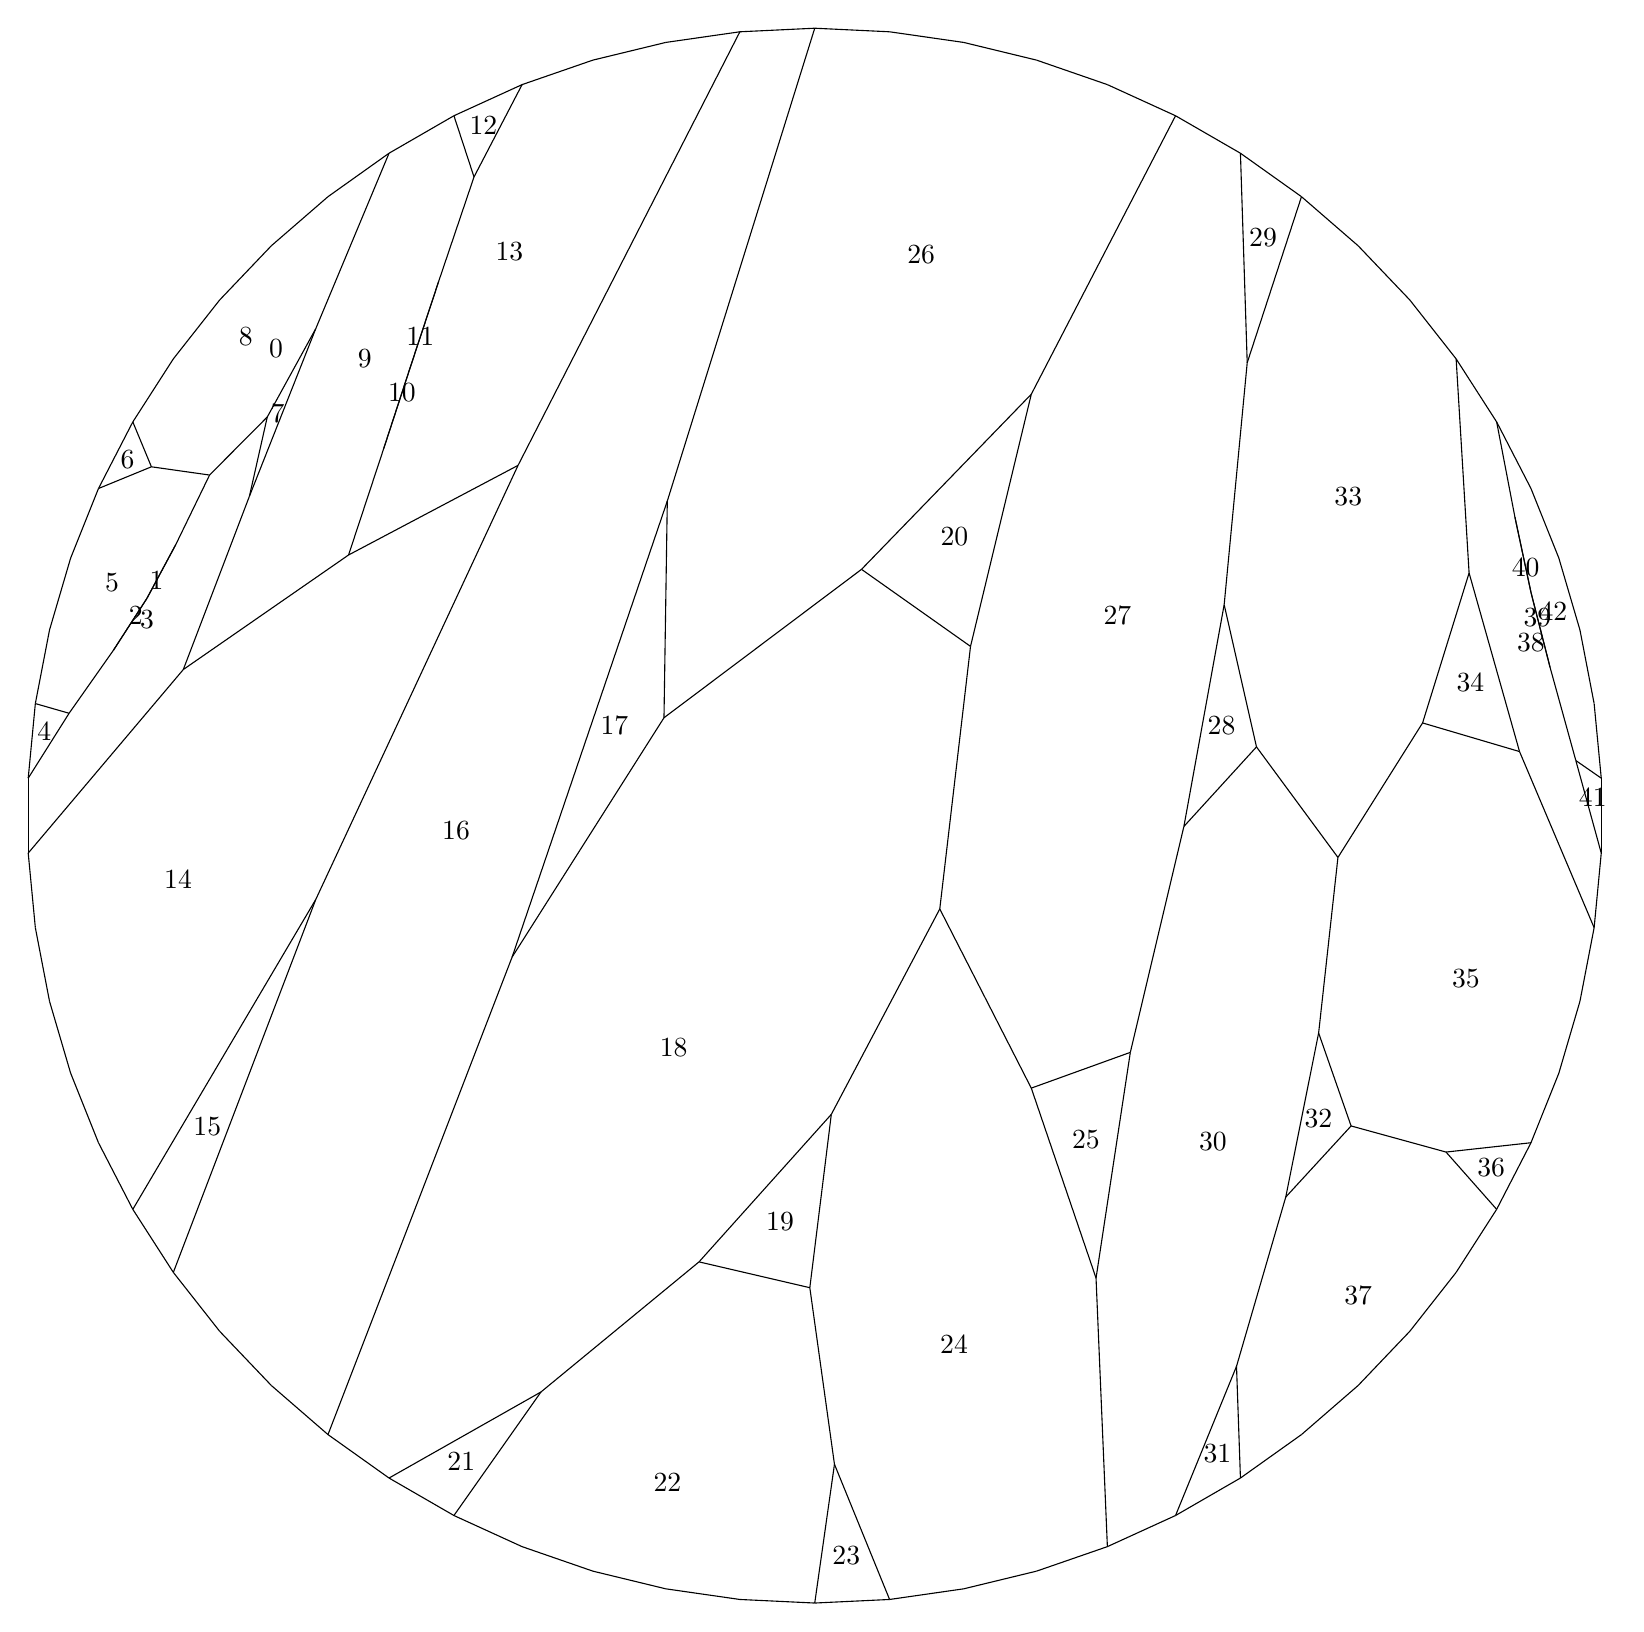
\begin{tikzpicture}[scale = 10, auto]
\coordinate (x0) at (-0.848192, 0.275787);
\coordinate (x1) at (-0.848192, 0.275787);
\coordinate (x2) at (-0.811383, 0.344377);
\coordinate (x3) at (-0.890438, 0.210336);
\coordinate (x4) at (-0.946964, 0.129992);
\coordinate (x5) at (-0.998867, 0.047582);
\coordinate (x6) at (-0.998867, -0.047582);
\coordinate (x7) at (-0.801909, 0.185524);
\coordinate (x8) at (-0.717923, 0.405637);
\coordinate (x9) at (-0.695270, 0.506283);
\coordinate (x10) at (-0.768539, 0.432537);
\coordinate (x11) at (-0.989821, 0.142315);
\coordinate (x12) at (-0.842414, 0.443009);
\coordinate (x13) at (-0.909632, 0.415415);
\coordinate (x14) at (-0.945001, 0.327068);
\coordinate (x15) at (-0.971812, 0.235759);
\coordinate (x16) at (-0.866025, 0.500000);
\coordinate (x17) at (-0.633684, 0.618459);
\coordinate (x18) at (-0.540641, 0.841254);
\coordinate (x19) at (-0.618159, 0.786053);
\coordinate (x20) at (-0.690079, 0.723734);
\coordinate (x21) at (-0.755750, 0.654861);
\coordinate (x22) at (-0.814576, 0.580057);
\coordinate (x23) at (-0.592048, 0.331009);
\coordinate (x24) at (-0.547488, 0.465891);
\coordinate (x25) at (-0.512560, 0.572744);
\coordinate (x26) at (-0.477567, 0.678540);
\coordinate (x27) at (-0.432725, 0.811127);
\coordinate (x28) at (-0.458227, 0.888835);
\coordinate (x29) at (-0.512560, 0.572744);
\coordinate (x30) at (-0.371662, 0.928368);
\coordinate (x31) at (-0.376795, 0.444815);
\coordinate (x32) at (-0.095056, 0.995472);
\coordinate (x33) at (-0.189251, 0.981929);
\coordinate (x34) at (-0.281733, 0.959493);
\coordinate (x35) at (-0.989821, -0.142315);
\coordinate (x36) at (-0.971812, -0.235759);
\coordinate (x37) at (-0.945001, -0.327068);
\coordinate (x38) at (-0.909632, -0.415415);
\coordinate (x39) at (-0.866025, -0.500000);
\coordinate (x40) at (-0.633673, -0.106447);
\coordinate (x41) at (-0.814576, -0.580057);
\coordinate (x42) at (-0.755750, -0.654861);
\coordinate (x43) at (-0.690079, -0.723734);
\coordinate (x44) at (-0.618159, -0.786053);
\coordinate (x45) at (-0.384345, -0.179661);
\coordinate (x46) at (-0.187239, 0.399502);
\coordinate (x47) at (0.000000, 1.000000);
\coordinate (x48) at (-0.191448, 0.124305);
\coordinate (x49) at (-0.540641, -0.841254);
\coordinate (x50) at (-0.347712, -0.731977);
\coordinate (x51) at (-0.146937, -0.566728);
\coordinate (x52) at (0.021058, -0.379395);
\coordinate (x53) at (0.158792, -0.118539);
\coordinate (x54) at (0.197842, 0.214930);
\coordinate (x55) at (0.059411, 0.312769);
\coordinate (x56) at (-0.006243, -0.599512);
\coordinate (x57) at (0.275020, 0.535177);
\coordinate (x58) at (-0.458227, -0.888835);
\coordinate (x59) at (-0.371662, -0.928368);
\coordinate (x60) at (-0.281733, -0.959493);
\coordinate (x61) at (-0.189251, -0.981929);
\coordinate (x62) at (-0.095056, -0.995472);
\coordinate (x63) at (-0.000000, -1.000000);
\coordinate (x64) at (0.025059, -0.823799);
\coordinate (x65) at (0.095056, -0.995472);
\coordinate (x66) at (0.189251, -0.981929);
\coordinate (x67) at (0.281733, -0.959493);
\coordinate (x68) at (0.371662, -0.928368);
\coordinate (x69) at (0.357257, -0.587304);
\coordinate (x70) at (0.275028, -0.346065);
\coordinate (x71) at (0.400807, -0.300641);
\coordinate (x72) at (0.458227, 0.888835);
\coordinate (x73) at (0.371662, 0.928368);
\coordinate (x74) at (0.281733, 0.959493);
\coordinate (x75) at (0.189251, 0.981929);
\coordinate (x76) at (0.095056, 0.995472);
\coordinate (x77) at (0.468827, -0.013734);
\coordinate (x78) at (0.519981, 0.267876);
\coordinate (x79) at (0.549236, 0.575166);
\coordinate (x80) at (0.540641, 0.841254);
\coordinate (x81) at (0.561017, 0.087293);
\coordinate (x82) at (0.618159, 0.786053);
\coordinate (x83) at (0.458227, -0.888835);
\coordinate (x84) at (0.535654, -0.699326);
\coordinate (x85) at (0.598196, -0.484402);
\coordinate (x86) at (0.639935, -0.276047);
\coordinate (x87) at (0.664466, -0.053100);
\coordinate (x88) at (0.540641, -0.841254);
\coordinate (x89) at (0.681173, -0.394111);
\coordinate (x90) at (0.771956, 0.117723);
\coordinate (x91) at (0.831022, 0.308177);
\coordinate (x92) at (0.814576, 0.580057);
\coordinate (x93) at (0.755750, 0.654861);
\coordinate (x94) at (0.690079, 0.723734);
\coordinate (x95) at (0.895079, 0.081366);
\coordinate (x96) at (0.801738, -0.427259);
\coordinate (x97) at (0.909632, -0.415415);
\coordinate (x98) at (0.945001, -0.327068);
\coordinate (x99) at (0.971812, -0.235759);
\coordinate (x100) at (0.989821, -0.142315);
\coordinate (x101) at (0.866025, -0.500000);
\coordinate (x102) at (0.618159, -0.786053);
\coordinate (x103) at (0.690079, -0.723734);
\coordinate (x104) at (0.755750, -0.654861);
\coordinate (x105) at (0.814576, -0.580057);
\coordinate (x106) at (0.998867, -0.047582);
\coordinate (x107) at (0.966576, 0.069967);
\coordinate (x108) at (0.933805, 0.188546);
\coordinate (x109) at (0.909686, 0.283219);
\coordinate (x110) at (0.889274, 0.378876);
\coordinate (x111) at (0.866025, 0.500000);
\coordinate (x112) at (0.909689, 0.283220);
\coordinate (x113) at (0.998867, 0.047582);
\coordinate (x114) at (0.989821, 0.142315);
\coordinate (x115) at (0.971812, 0.235759);
\coordinate (x116) at (0.945001, 0.327068);
\coordinate (x117) at (0.909632, 0.415415);
\draw (-0.848192, 0.275787) -- (-0.848192, 0.275787);
\draw (-0.848192, 0.275787) -- (-0.811383, 0.344377);
\draw (-0.811383, 0.344377) -- (-0.848192, 0.275787);
\draw (-0.848192, 0.275787) -- (-0.890438, 0.210336);
\draw (-0.890438, 0.210336) -- (-0.848192, 0.275787);
\draw (-0.890438, 0.210336) -- (-0.946964, 0.129992);
\draw (-0.946964, 0.129992) -- (-0.998867, 0.047582);
\draw (-0.998867, 0.047582) -- (-0.998867, -0.047582);
\draw (-0.998867, -0.047582) -- (-0.801909, 0.185524);
\draw (-0.801909, 0.185524) -- (-0.717923, 0.405637);
\draw (-0.717923, 0.405637) -- (-0.695270, 0.506283);
\draw (-0.695270, 0.506283) -- (-0.768539, 0.432537);
\draw (-0.768539, 0.432537) -- (-0.811383, 0.344377);
\draw (-0.946964, 0.129992) -- (-0.989821, 0.142315);
\draw (-0.989821, 0.142315) -- (-0.998867, 0.047582);
\draw (-0.768539, 0.432537) -- (-0.842414, 0.443009);
\draw (-0.842414, 0.443009) -- (-0.909632, 0.415415);
\draw (-0.909632, 0.415415) -- (-0.945001, 0.327068);
\draw (-0.945001, 0.327068) -- (-0.971812, 0.235759);
\draw (-0.971812, 0.235759) -- (-0.989821, 0.142315);
\draw (-0.842414, 0.443009) -- (-0.866025, 0.500000);
\draw (-0.866025, 0.500000) -- (-0.909632, 0.415415);
\draw (-0.717923, 0.405637) -- (-0.633684, 0.618459);
\draw (-0.633684, 0.618459) -- (-0.695270, 0.506283);
\draw (-0.633684, 0.618459) -- (-0.540641, 0.841254);
\draw (-0.540641, 0.841254) -- (-0.618159, 0.786053);
\draw (-0.618159, 0.786053) -- (-0.690079, 0.723734);
\draw (-0.690079, 0.723734) -- (-0.755750, 0.654861);
\draw (-0.755750, 0.654861) -- (-0.814576, 0.580057);
\draw (-0.814576, 0.580057) -- (-0.866025, 0.500000);
\draw (-0.801909, 0.185524) -- (-0.592048, 0.331009);
\draw (-0.592048, 0.331009) -- (-0.547488, 0.465891);
\draw (-0.547488, 0.465891) -- (-0.512560, 0.572744);
\draw (-0.512560, 0.572744) -- (-0.477567, 0.678540);
\draw (-0.477567, 0.678540) -- (-0.432725, 0.811127);
\draw (-0.432725, 0.811127) -- (-0.458227, 0.888835);
\draw (-0.458227, 0.888835) -- (-0.540641, 0.841254);
\draw (-0.547488, 0.465891) -- (-0.512560, 0.572744);
\draw (-0.512560, 0.572744) -- (-0.512560, 0.572744);
\draw (-0.512560, 0.572744) -- (-0.477567, 0.678540);
\draw (-0.432725, 0.811127) -- (-0.371662, 0.928368);
\draw (-0.371662, 0.928368) -- (-0.458227, 0.888835);
\draw (-0.592048, 0.331009) -- (-0.376795, 0.444815);
\draw (-0.376795, 0.444815) -- (-0.095056, 0.995472);
\draw (-0.095056, 0.995472) -- (-0.189251, 0.981929);
\draw (-0.189251, 0.981929) -- (-0.281733, 0.959493);
\draw (-0.281733, 0.959493) -- (-0.371662, 0.928368);
\draw (-0.998867, -0.047582) -- (-0.989821, -0.142315);
\draw (-0.989821, -0.142315) -- (-0.971812, -0.235759);
\draw (-0.971812, -0.235759) -- (-0.945001, -0.327068);
\draw (-0.945001, -0.327068) -- (-0.909632, -0.415415);
\draw (-0.909632, -0.415415) -- (-0.866025, -0.500000);
\draw (-0.866025, -0.500000) -- (-0.633673, -0.106447);
\draw (-0.633673, -0.106447) -- (-0.376795, 0.444815);
\draw (-0.866025, -0.500000) -- (-0.814576, -0.580057);
\draw (-0.814576, -0.580057) -- (-0.633673, -0.106447);
\draw (-0.814576, -0.580057) -- (-0.755750, -0.654861);
\draw (-0.755750, -0.654861) -- (-0.690079, -0.723734);
\draw (-0.690079, -0.723734) -- (-0.618159, -0.786053);
\draw (-0.618159, -0.786053) -- (-0.384345, -0.179661);
\draw (-0.384345, -0.179661) -- (-0.187239, 0.399502);
\draw (-0.187239, 0.399502) -- (0.000000, 1.000000);
\draw (0.000000, 1.000000) -- (-0.095056, 0.995472);
\draw (-0.384345, -0.179661) -- (-0.191448, 0.124305);
\draw (-0.191448, 0.124305) -- (-0.187239, 0.399502);
\draw (-0.618159, -0.786053) -- (-0.540641, -0.841254);
\draw (-0.540641, -0.841254) -- (-0.347712, -0.731977);
\draw (-0.347712, -0.731977) -- (-0.146937, -0.566728);
\draw (-0.146937, -0.566728) -- (0.021058, -0.379395);
\draw (0.021058, -0.379395) -- (0.158792, -0.118539);
\draw (0.158792, -0.118539) -- (0.197842, 0.214930);
\draw (0.197842, 0.214930) -- (0.059411, 0.312769);
\draw (0.059411, 0.312769) -- (-0.191448, 0.124305);
\draw (-0.146937, -0.566728) -- (-0.006243, -0.599512);
\draw (-0.006243, -0.599512) -- (0.021058, -0.379395);
\draw (0.197842, 0.214930) -- (0.275020, 0.535177);
\draw (0.275020, 0.535177) -- (0.059411, 0.312769);
\draw (-0.540641, -0.841254) -- (-0.458227, -0.888835);
\draw (-0.458227, -0.888835) -- (-0.347712, -0.731977);
\draw (-0.458227, -0.888835) -- (-0.371662, -0.928368);
\draw (-0.371662, -0.928368) -- (-0.281733, -0.959493);
\draw (-0.281733, -0.959493) -- (-0.189251, -0.981929);
\draw (-0.189251, -0.981929) -- (-0.095056, -0.995472);
\draw (-0.095056, -0.995472) -- (-0.000000, -1.000000);
\draw (-0.000000, -1.000000) -- (0.025059, -0.823799);
\draw (0.025059, -0.823799) -- (-0.006243, -0.599512);
\draw (-0.000000, -1.000000) -- (0.095056, -0.995472);
\draw (0.095056, -0.995472) -- (0.025059, -0.823799);
\draw (0.095056, -0.995472) -- (0.189251, -0.981929);
\draw (0.189251, -0.981929) -- (0.281733, -0.959493);
\draw (0.281733, -0.959493) -- (0.371662, -0.928368);
\draw (0.371662, -0.928368) -- (0.357257, -0.587304);
\draw (0.357257, -0.587304) -- (0.275028, -0.346065);
\draw (0.275028, -0.346065) -- (0.158792, -0.118539);
\draw (0.357257, -0.587304) -- (0.400807, -0.300641);
\draw (0.400807, -0.300641) -- (0.275028, -0.346065);
\draw (0.275020, 0.535177) -- (0.458227, 0.888835);
\draw (0.458227, 0.888835) -- (0.371662, 0.928368);
\draw (0.371662, 0.928368) -- (0.281733, 0.959493);
\draw (0.281733, 0.959493) -- (0.189251, 0.981929);
\draw (0.189251, 0.981929) -- (0.095056, 0.995472);
\draw (0.095056, 0.995472) -- (0.000000, 1.000000);
\draw (0.400807, -0.300641) -- (0.468827, -0.013734);
\draw (0.468827, -0.013734) -- (0.519981, 0.267876);
\draw (0.519981, 0.267876) -- (0.549236, 0.575166);
\draw (0.549236, 0.575166) -- (0.540641, 0.841254);
\draw (0.540641, 0.841254) -- (0.458227, 0.888835);
\draw (0.468827, -0.013734) -- (0.561017, 0.087293);
\draw (0.561017, 0.087293) -- (0.519981, 0.267876);
\draw (0.549236, 0.575166) -- (0.618159, 0.786053);
\draw (0.618159, 0.786053) -- (0.540641, 0.841254);
\draw (0.371662, -0.928368) -- (0.458227, -0.888835);
\draw (0.458227, -0.888835) -- (0.535654, -0.699326);
\draw (0.535654, -0.699326) -- (0.598196, -0.484402);
\draw (0.598196, -0.484402) -- (0.639935, -0.276047);
\draw (0.639935, -0.276047) -- (0.664466, -0.053100);
\draw (0.664466, -0.053100) -- (0.561017, 0.087293);
\draw (0.458227, -0.888835) -- (0.540641, -0.841254);
\draw (0.540641, -0.841254) -- (0.535654, -0.699326);
\draw (0.598196, -0.484402) -- (0.681173, -0.394111);
\draw (0.681173, -0.394111) -- (0.639935, -0.276047);
\draw (0.664466, -0.053100) -- (0.771956, 0.117723);
\draw (0.771956, 0.117723) -- (0.831022, 0.308177);
\draw (0.831022, 0.308177) -- (0.814576, 0.580057);
\draw (0.814576, 0.580057) -- (0.755750, 0.654861);
\draw (0.755750, 0.654861) -- (0.690079, 0.723734);
\draw (0.690079, 0.723734) -- (0.618159, 0.786053);
\draw (0.771956, 0.117723) -- (0.895079, 0.081366);
\draw (0.895079, 0.081366) -- (0.831022, 0.308177);
\draw (0.681173, -0.394111) -- (0.801738, -0.427259);
\draw (0.801738, -0.427259) -- (0.909632, -0.415415);
\draw (0.909632, -0.415415) -- (0.945001, -0.327068);
\draw (0.945001, -0.327068) -- (0.971812, -0.235759);
\draw (0.971812, -0.235759) -- (0.989821, -0.142315);
\draw (0.989821, -0.142315) -- (0.895079, 0.081366);
\draw (0.801738, -0.427259) -- (0.866025, -0.500000);
\draw (0.866025, -0.500000) -- (0.909632, -0.415415);
\draw (0.540641, -0.841254) -- (0.618159, -0.786053);
\draw (0.618159, -0.786053) -- (0.690079, -0.723734);
\draw (0.690079, -0.723734) -- (0.755750, -0.654861);
\draw (0.755750, -0.654861) -- (0.814576, -0.580057);
\draw (0.814576, -0.580057) -- (0.866025, -0.500000);
\draw (0.989821, -0.142315) -- (0.998867, -0.047582);
\draw (0.998867, -0.047582) -- (0.966576, 0.069967);
\draw (0.966576, 0.069967) -- (0.933805, 0.188546);
\draw (0.933805, 0.188546) -- (0.909686, 0.283219);
\draw (0.909686, 0.283219) -- (0.889274, 0.378876);
\draw (0.889274, 0.378876) -- (0.866025, 0.500000);
\draw (0.866025, 0.500000) -- (0.814576, 0.580057);
\draw (0.933805, 0.188546) -- (0.909689, 0.283220);
\draw (0.909689, 0.283220) -- (0.909686, 0.283219);
\draw (0.909689, 0.283220) -- (0.889274, 0.378876);
\draw (0.998867, -0.047582) -- (0.998867, 0.047582);
\draw (0.998867, 0.047582) -- (0.966576, 0.069967);
\draw (0.998867, 0.047582) -- (0.989821, 0.142315);
\draw (0.989821, 0.142315) -- (0.971812, 0.235759);
\draw (0.971812, 0.235759) -- (0.945001, 0.327068);
\draw (0.945001, 0.327068) -- (0.909632, 0.415415);
\draw (0.909632, 0.415415) -- (0.866025, 0.500000);
\node at (-0.684262, 0.592917) {0};
\node at (-0.835922, 0.298650) {1};
\node at (-0.862274, 0.253970) {2};
\node at (-0.847835, 0.249047) {3};
\node at (-0.978551, 0.106629) {4};
\node at (-0.892420, 0.295659) {5};
\node at (-0.872690, 0.452808) {6};
\node at (-0.682292, 0.510126) {7};
\node at (-0.722514, 0.608625) {8};
\node at (-0.571477, 0.579902) {9};
\node at (-0.524202, 0.537126) {10};
\node at (-0.500895, 0.608009) {11};
\node at (-0.420871, 0.876110) {12};
\node at (-0.387688, 0.716939) {13};
\node at (-0.808558, -0.081324) {14};
\node at (-0.771425, -0.395501) {15};
\node at (-0.455567, -0.019102) {16};
\node at (-0.254344, 0.114715) {17};
\node at (-0.179214, -0.295160) {18};
\node at (-0.044041, -0.515212) {19};
\node at (0.177424, 0.354292) {20};
\node at (-0.448860, -0.820689) {21};
\node at (-0.187176, -0.847611) {22};
\node at (0.040038, -0.939757) {23};
\node at (0.176865, -0.671988) {24};
\node at (0.344364, -0.411337) {25};
\node at (0.135167, 0.712585) {26};
\node at (0.384440, 0.254426) {27};
\node at (0.516609, 0.113811) {28};
\node at (0.569345, 0.734158) {29};
\node at (0.505605, -0.414446) {30};
\node at (0.511507, -0.809805) {31};
\node at (0.639768, -0.384853) {32};
\node at (0.677624, 0.404784) {33};
\node at (0.832686, 0.169088) {34};
\node at (0.827061, -0.207198) {35};
\node at (0.859132, -0.447558) {36};
\node at (0.690199, -0.609106) {37};
\node at (0.909473, 0.220031) {38};
\node at (0.917727, 0.251661) {39};
\node at (0.902883, 0.315105) {40};
\node at (0.988103, 0.023322) {41};
\node at (0.938050, 0.258875) {42};
\end{tikzpicture}
\caption{Graph}

\end{figure}
\end{document}

        \end{scope}
        \\
      };
    \end{tikzfigure}
    \begin{tikzfigure}{\label{fig:expansion:patch:poly:3:10}}{\todo{caption, rework patch}}

      \matrix (m) [column sep=1cm] {
        % \begin{scope}[scale=3]
        %   \coordinate (x0) at (0.149611, -0.683175);
\coordinate (x1) at (-0.093312, -0.648545);
\coordinate (x2) at (-0.336047, -0.613347);
\coordinate (x3) at (-0.841254, -0.540641);
\coordinate (x4) at (-0.415415, -0.909632);
\coordinate (x5) at (0.142315, -0.989821);
\coordinate (x6) at (0.654861, -0.755750);
\coordinate (x7) at (0.959493, -0.281733);
\coordinate (x8) at (0.662341, -0.000000);
\coordinate (x9) at (0.198819, -0.000000);
\coordinate (x10) at (-0.169004, 0.000000);
\coordinate (x11) at (-0.536781, 0.000000);
\coordinate (x12) at (-1.000000, 0.000000);
\coordinate (x13) at (-0.169004, 0.000000);
\coordinate (x14) at (0.959493, 0.281733);
\coordinate (x15) at (0.654861, 0.755750);
\coordinate (x16) at (0.142315, 0.989821);
\coordinate (x17) at (-0.415415, 0.909632);
\coordinate (x18) at (-0.841254, 0.540641);
\draw (0.149611, -0.683175) -- (-0.093312, -0.648545);
\draw (-0.093312, -0.648545) -- (-0.336047, -0.613347);
\draw (-0.336047, -0.613347) -- (-0.841254, -0.540641);
\draw (-0.841254, -0.540641) -- (-0.415415, -0.909632);
\draw (-0.415415, -0.909632) -- (0.142315, -0.989821);
\draw (0.142315, -0.989821) -- (0.654861, -0.755750);
\draw (0.654861, -0.755750) -- (0.149611, -0.683175);
\draw (0.149611, -0.683175) -- (-0.336047, -0.613347);
\draw (0.654861, -0.755750) -- (0.959493, -0.281733);
\draw (0.959493, -0.281733) -- (0.662341, -0.000000);
\draw (0.662341, -0.000000) -- (0.198819, -0.000000);
\draw (0.198819, -0.000000) -- (-0.169004, 0.000000);
\draw (-0.169004, 0.000000) -- (-0.536781, 0.000000);
\draw (-0.536781, 0.000000) -- (-1.000000, 0.000000);
\draw (-1.000000, 0.000000) -- (-0.841254, -0.540641);
\draw (0.198819, -0.000000) -- (-0.169004, 0.000000);
\draw (-0.169004, 0.000000) -- (-0.169004, 0.000000);
\draw (-0.169004, 0.000000) -- (-0.536781, 0.000000);
\draw (0.959493, -0.281733) -- (0.959493, 0.281733);
\draw (0.959493, 0.281733) -- (0.662341, -0.000000);
\draw (0.959493, 0.281733) -- (0.654861, 0.755750);
\draw (0.654861, 0.755750) -- (0.142315, 0.989821);
\draw (0.142315, 0.989821) -- (-0.415415, 0.909632);
\draw (-0.415415, 0.909632) -- (-0.841254, 0.540641);
\draw (-0.841254, 0.540641) -- (-1.000000, 0.000000);

        % \end{scope}
        \begin{scope}[yscale=0.866, scale=0.7]
          \draw[very thick] (0.5,1)--(-0.5,1)--(-4,6.667)--(-3.5,11.5)--(-2.5,12)--(-1.5,12)--(-0.5,11.5)--(-0.5,12.5)--(0.5,13.5)--(0.5,14.5)--(1.5,14)-- (2.5,14)--(3.5,14.5)--(3.5,13.5)--(4.5,12.5)--(5.5,12.5)--(6.5,13)--(7.375, 12.25)--(7.875, 11.25)--(7.625, 9.75)-- (6.875, 9.25)-- (3,7.333)--(0.5,1);
          \draw (-0.5,11.5)--(2,9)--(3,9)--(4.5,11.5)--(4.5,12.5);
          \draw (4.5,11.5)--(5.5,12.5);
          \draw (3,7.333)--(2.75,8)--(2,9);
          \draw (2.75,8)--(3,9);
          \draw (0.5,13.5)--(1.5,14);
          \draw (2.5,14)--(3.5,13.5);

          \node[anchor=135] at (0.5,1)        {$i_{0}'$};
          \node[anchor= 45] at (-0.5,1)       {$i_0$};
          \node[anchor=225] at (-4,6.667)     {$i_1$};
          \node[anchor=330] at (-3.5,11.5)    {$i_2$};
          \node[anchor=270] at (-2.5,12)      {$i_{3}=o_0$};
          \node[anchor= 90] at (-1.5,12)      {$o_{1}$};
          \node[anchor= 90] at (-0.5,11.5)    {$o_{2}$};
          \node[anchor=315] at (-0.5,12.5)    {$o_{3}$};
          \node[anchor=335] at (0.5,13.5)     {$o_{4}$};
          \node[anchor=270] at (0.5,14.5)     {$o_{5}$};
          \node[anchor= 90] at (1.5,14)       {$o_{6}$};
          \node[anchor= 90] at (2.5,14)       {$o_{7}$};
          \node[anchor=270] at (3.5,14.5)     {$o_8$};
          \node[anchor=205] at (3.5,13.5)     {$o_{9}$}; 
          \node[anchor=235] at (4.5,12.5)     {$o_{10}$};
          \node[anchor=270] at (5.5,12.5)     {$o_{11}$};
          \node[anchor=270] at (6.5,13)       {$\mathbf{o_{12}}$};
          \node[anchor=235] at (7.375, 12.25) {$o_{13}$};
          \node[anchor=180] at (7.875, 11.25) {$o_{14}$};
          \node[anchor=160] at (7.625, 9.75)  {$i_3'=o_{15}$};
          \node[anchor=140] at (6.875, 9.25)  {$i_2'$};
          \node[anchor=340] at (3,7.333)      {$i_1'$};

          \fill[black] (0.5,1)        circle (2pt); 
          \fill[black] (-0.5,1)       circle (2pt);
          \fill[black] (-4,6.667)     circle (2pt);
          \fill[black] (-3.5,11.5)    circle (2pt);
          \fill[black] (-2.5,12)      circle (2pt);
          \fill[black] (-1.5,12)      circle (2pt);
          \fill[black] (-0.5,11.5)    circle (2pt);
          \fill[black] (-0.5,12.5)    circle (2pt);
          \fill[black] (0.5,13.5)     circle (2pt);
          \fill[black] (0.5,14.5)     circle (2pt);
          \fill[black] (1.5,14)       circle (2pt);
          \fill[black] (2.5,14)       circle (2pt);
          \fill[black] (3.5,14.5)     circle (2pt);
          \fill[black] (3.5,13.5)     circle (2pt);
          \fill[black] (4.5,12.5)     circle (2pt);
          \fill[black] (5.5,12.5)     circle (2pt);
          \fill[black] (6.5,13)       circle (2pt);
          \fill[black] (7.375, 12.25) circle (2pt);
          \fill[black] (7.875, 11.25) circle (2pt);
          \fill[black] (7.625, 9.75)  circle (2pt);
          \fill[black] (6.875, 9.25)  circle (2pt);
          \fill[black] (3,7.333)      circle (2pt);
          \fill[black] (2.75,8)       circle (2pt);
          \fill[black] (2,9)          circle (2pt);
          \fill[black] (4.5,11.5)     circle (2pt);
          \fill[black] (3,9)          circle (2pt);
          
          \node at (-0.5,8)  {$10$};
          \node at (2,12)   {$10$};
          \node at (5.5,10) {$10$};
          \node at (2.6,8.6) {$3$};
          \node at (0.833,14) {$3$};
          \node at (3.166,14){$3$};
          \node at (4.833,12.2){$3$};

        \end{scope}
        &
        \begin{scope}[scale=0.4]
          \begin{scope}[yscale=0.866]
            \draw[very thick] (0.5,1)--(-0.5,1)--(-4,6.667)--(-3.5,11.5)--(-2.5,12)--(-1.5,12)--(-0.5,11.5)--(-0.5,12.5)--(0.5,13.5)--(0.5,14.5)--(1.5,14)-- (2.5,14)--(3.5,14.5)--(3.5,13.5)--(4.5,12.5)--(5.5,12.5)--(6.5,13)--(7.375, 12.25)--(7.875, 11.25)--(7.625, 9.75)-- (6.875, 9.25)-- (3,7.333)--(0.5,1);
            \draw (-0.5,11.5)--(2,9)--(3,9)--(4.5,11.5)--(4.5,12.5);
            \draw (4.5,11.5)--(5.5,12.5);
            \draw (3,7.333)--(2.75,8)--(2,9);
            \draw (2.75,8)--(3,9);
            \draw (0.5,13.5)--(1.5,14);
            \draw (2.5,14)--(3.5,13.5);

            \fill[black] (0.5,1)        circle (3pt); 
          \fill[black] (-0.5,1)       circle (3pt);
          \fill[black] (-4,6.667)     circle (3pt);
          \fill[black] (-3.5,11.5)    circle (3pt);
          \fill[black] (-2.5,12)      circle (3pt);
          \fill[black] (-1.5,12)      circle (3pt);
          \fill[black] (-0.5,11.5)    circle (3pt);
          \fill[black] (-0.5,12.5)    circle (3pt);
          \fill[black] (0.5,13.5)     circle (3pt);
          \fill[black] (0.5,14.5)     circle (3pt);
          \fill[black] (1.5,14)       circle (3pt);
          \fill[black] (2.5,14)       circle (3pt);
          \fill[black] (3.5,14.5)     circle (3pt);
          \fill[black] (3.5,13.5)     circle (3pt);
          \fill[black] (4.5,12.5)     circle (3pt);
          \fill[black] (5.5,12.5)     circle (3pt);
          \fill[black] (6.5,13)       circle (3pt);
          \fill[black] (7.375, 12.25) circle (3pt);
          \fill[black] (7.875, 11.25) circle (3pt);
          \fill[black] (7.625, 9.75)  circle (3pt);
          \fill[black] (6.875, 9.25)  circle (3pt);
          \fill[black] (3,7.333)      circle (3pt);
          \fill[black] (2.75,8)       circle (3pt);
          \fill[black] (2,9)          circle (3pt);
          \fill[black] (4.5,11.5)     circle (3pt);
          \fill[black] (3,9)          circle (3pt);
            
          \end{scope}
          \begin{scope}[rotate=60, yscale=0.866]
            \draw[very thick] (0.5,1)--(-0.5,1)--(-4,6.667)--(-3.5,11.5)--(-2.5,12)--(-1.5,12)--(-0.5,11.5)--(-0.5,12.5)--(0.5,13.5)--(0.5,14.5)--(1.5,14)-- (2.5,14)--(3.5,14.5)--(3.5,13.5)--(4.5,12.5)--(5.5,12.5)--(6.5,13)--(7.375, 12.25)--(7.875, 11.25)--(7.625, 9.75)-- (6.875, 9.25)-- (3,7.333)--(0.5,1);
            \draw (-0.5,11.5)--(2,9)--(3,9)--(4.5,11.5)--(4.5,12.5);
            \draw (4.5,11.5)--(5.5,12.5);
            \draw (3,7.333)--(2.75,8)--(2,9);
            \draw (2.75,8)--(3,9);
            \draw (0.5,13.5)--(1.5,14);
            \draw (2.5,14)--(3.5,13.5);

                        \fill[black] (0.5,1)        circle (3pt); 
          \fill[black] (-0.5,1)       circle (3pt);
          \fill[black] (-4,6.667)     circle (3pt);
          \fill[black] (-3.5,11.5)    circle (3pt);
          \fill[black] (-2.5,12)      circle (3pt);
          \fill[black] (-1.5,12)      circle (3pt);
          \fill[black] (-0.5,11.5)    circle (3pt);
          \fill[black] (-0.5,12.5)    circle (3pt);
          \fill[black] (0.5,13.5)     circle (3pt);
          \fill[black] (0.5,14.5)     circle (3pt);
          \fill[black] (1.5,14)       circle (3pt);
          \fill[black] (2.5,14)       circle (3pt);
          \fill[black] (3.5,14.5)     circle (3pt);
          \fill[black] (3.5,13.5)     circle (3pt);
          \fill[black] (4.5,12.5)     circle (3pt);
          \fill[black] (5.5,12.5)     circle (3pt);
          \fill[black] (6.5,13)       circle (3pt);
          \fill[black] (7.375, 12.25) circle (3pt);
          \fill[black] (7.875, 11.25) circle (3pt);
          \fill[black] (7.625, 9.75)  circle (3pt);
          \fill[black] (6.875, 9.25)  circle (3pt);
          \fill[black] (3,7.333)      circle (3pt);
\fill[black] (2.75,8)       circle (3pt);
          \fill[black] (2,9)          circle (3pt);
          \fill[black] (4.5,11.5)     circle (3pt);
          \fill[black] (3,9)          circle (3pt);
          
          \end{scope}
          \begin{scope}[yscale=0.866,shift={(0 cm,26 cm)},rotate=180]
            \draw[very thick] (0.5,1)--(-0.5,1)--(-4,6.667)--(-3.5,11.5)--(-2.5,12)--(-1.5,12)--(-0.5,11.5)--(-0.5,12.5)--(0.5,13.5)--(0.5,14.5)--(1.5,14)-- (2.5,14)--(3.5,14.5)--(3.5,13.5)--(4.5,12.5)--(5.5,12.5)--(6.5,13)--(7.375, 12.25)--(7.875, 11.25)--(7.625, 9.75)-- (6.875, 9.25)-- (3,7.333)--(0.5,1);
            \draw (-0.5,11.5)--(2,9)--(3,9)--(4.5,11.5)--(4.5,12.5);
            \draw (4.5,11.5)--(5.5,12.5);
            \draw (3,7.333)--(2.75,8)--(2,9);
            \draw (2.75,8)--(3,9);
            \draw (0.5,13.5)--(1.5,14);
            \draw (2.5,14)--(3.5,13.5);

                        \fill[black] (0.5,1)        circle (3pt); 
          \fill[black] (-0.5,1)       circle (3pt);
          \fill[black] (-4,6.667)     circle (3pt);
          \fill[black] (-3.5,11.5)    circle (3pt);
          \fill[black] (-2.5,12)      circle (3pt);
          \fill[black] (-1.5,12)      circle (3pt);
          \fill[black] (-0.5,11.5)    circle (3pt);
          \fill[black] (-0.5,12.5)    circle (3pt);
          \fill[black] (0.5,13.5)     circle (3pt);
          \fill[black] (0.5,14.5)     circle (3pt);
          \fill[black] (1.5,14)       circle (3pt);
          \fill[black] (2.5,14)       circle (3pt);
          \fill[black] (3.5,14.5)     circle (3pt);
          \fill[black] (3.5,13.5)     circle (3pt);
          \fill[black] (4.5,12.5)     circle (3pt);
          \fill[black] (5.5,12.5)     circle (3pt);
          \fill[black] (6.5,13)       circle (3pt);
          \fill[black] (7.375, 12.25) circle (3pt);
          \fill[black] (7.875, 11.25) circle (3pt);
          \fill[black] (7.625, 9.75)  circle (3pt);
          \fill[black] (6.875, 9.25)  circle (3pt);
          \fill[black] (3,7.333)      circle (3pt);
\fill[black] (2.75,8)       circle (3pt);
          \fill[black] (2,9)          circle (3pt);
          \fill[black] (4.5,11.5)     circle (3pt);
          \fill[black] (3,9)          circle (3pt);
          \end{scope}
          \begin{scope}[shift={(0 cm,22.516 cm)},rotate=240,yscale=0.866]
            \draw[very thick] (0.5,1)--(-0.5,1)--(-4,6.667)--(-3.5,11.5)--(-2.5,12)--(-1.5,12)--(-0.5,11.5)--(-0.5,12.5)--(0.5,13.5)--(0.5,14.5)--(1.5,14)-- (2.5,14)--(3.5,14.5)--(3.5,13.5)--(4.5,12.5)--(5.5,12.5)--(6.5,13)--(7.375, 12.25)--(7.875, 11.25)--(7.625, 9.75)-- (6.875, 9.25)-- (3,7.333)--(0.5,1);
            \draw (-0.5,11.5)--(2,9)--(3,9)--(4.5,11.5)--(4.5,12.5);
            \draw (4.5,11.5)--(5.5,12.5);
            \draw (3,7.333)--(2.75,8)--(2,9);
            \draw (2.75,8)--(3,9);
            \draw (0.5,13.5)--(1.5,14);
            \draw (2.5,14)--(3.5,13.5);

                        \fill[black] (0.5,1)        circle (3pt); 
          \fill[black] (-0.5,1)       circle (3pt);
          \fill[black] (-4,6.667)     circle (3pt);
          \fill[black] (-3.5,11.5)    circle (3pt);
          \fill[black] (-2.5,12)      circle (3pt);
          \fill[black] (-1.5,12)      circle (3pt);
          \fill[black] (-0.5,11.5)    circle (3pt);
          \fill[black] (-0.5,12.5)    circle (3pt);
          \fill[black] (0.5,13.5)     circle (3pt);
          \fill[black] (0.5,14.5)     circle (3pt);
          \fill[black] (1.5,14)       circle (3pt);
          \fill[black] (2.5,14)       circle (3pt);
          \fill[black] (3.5,14.5)     circle (3pt);
          \fill[black] (3.5,13.5)     circle (3pt);
          \fill[black] (4.5,12.5)     circle (3pt);
          \fill[black] (5.5,12.5)     circle (3pt);
          \fill[black] (6.5,13)       circle (3pt);
          \fill[black] (7.375, 12.25) circle (3pt);
          \fill[black] (7.875, 11.25) circle (3pt);
          \fill[black] (7.625, 9.75)  circle (3pt);
          \fill[black] (6.875, 9.25)  circle (3pt);
          \fill[black] (3,7.333)      circle (3pt);
\fill[black] (2.75,8)       circle (3pt);
          \fill[black] (2,9)          circle (3pt);
          \fill[black] (4.5,11.5)     circle (3pt);
          \fill[black] (3,9)          circle (3pt);
          \end{scope}
        \end{scope}
        \\
      };
      % \begin{scope}[scale=3]
      %   \documentclass[a4paper]{article}
\usepackage[left=0.5cm, right=0.5cm, top=1cm, bottom=1cm]{geometry}
\usepackage{tikz}
\begin{document}
\begin{figure}[h!]
\centering
\begin{tikzpicture}[scale = 10, auto]
\coordinate (x0) at (0.166104, 0.013310);
\coordinate (x1) at (0.138873, -0.202200);
\coordinate (x2) at (0.386369, -0.560024);
\coordinate (x3) at (0.748511, -0.663123);
\coordinate (x4) at (0.970942, -0.239316);
\coordinate (x5) at (0.794923, 0.001403);
\coordinate (x6) at (0.480588, 0.007178);
\coordinate (x7) at (-0.131665, 0.121253);
\coordinate (x8) at (0.354605, -0.935016);
\coordinate (x9) at (0.970942, 0.239316);
\coordinate (x10) at (0.748511, 0.663123);
\coordinate (x11) at (0.354605, 0.935016);
\coordinate (x12) at (-0.120537, 0.992709);
\coordinate (x13) at (-0.568065, 0.822984);
\coordinate (x14) at (-0.484996, 0.430986);
\coordinate (x15) at (-0.885456, 0.464723);
\coordinate (x16) at (-1.000000, 0.000000);
\coordinate (x17) at (-0.885456, -0.464723);
\coordinate (x18) at (-0.568065, -0.822984);
\coordinate (x19) at (-0.120537, -0.992709);
\draw (0.166104, 0.013310) -- (0.138873, -0.202200);
\draw (0.138873, -0.202200) -- (0.386369, -0.560024);
\draw (0.386369, -0.560024) -- (0.748511, -0.663123);
\draw (0.748511, -0.663123) -- (0.970942, -0.239316);
\draw (0.970942, -0.239316) -- (0.794923, 0.001403);
\draw (0.794923, 0.001403) -- (0.480588, 0.007178);
\draw (0.480588, 0.007178) -- (0.166104, 0.013310);
\draw (0.166104, 0.013310) -- (-0.131665, 0.121253);
\draw (-0.131665, 0.121253) -- (0.138873, -0.202200);
\draw (0.386369, -0.560024) -- (0.354605, -0.935016);
\draw (0.354605, -0.935016) -- (0.748511, -0.663123);
\draw (0.970942, -0.239316) -- (0.970942, 0.239316);
\draw (0.970942, 0.239316) -- (0.794923, 0.001403);
\draw (0.970942, 0.239316) -- (0.748511, 0.663123);
\draw (0.748511, 0.663123) -- (0.354605, 0.935016);
\draw (0.354605, 0.935016) -- (-0.120537, 0.992709);
\draw (-0.120537, 0.992709) -- (-0.568065, 0.822984);
\draw (-0.568065, 0.822984) -- (-0.484996, 0.430986);
\draw (-0.484996, 0.430986) -- (-0.131665, 0.121253);
\draw (-0.568065, 0.822984) -- (-0.885456, 0.464723);
\draw (-0.885456, 0.464723) -- (-0.484996, 0.430986);
\draw (-0.885456, 0.464723) -- (-1.000000, 0.000000);
\draw (-1.000000, 0.000000) -- (-0.885456, -0.464723);
\draw (-0.885456, -0.464723) -- (-0.568065, -0.822984);
\draw (-0.568065, -0.822984) -- (-0.120537, -0.992709);
\draw (-0.120537, -0.992709) -- (0.354605, -0.935016);
\node at (-0.000000, 0.000000) {0};
\node at (0.526616, -0.234682) {1};
\node at (0.057771, -0.022546) {2};
\node at (0.496495, -0.719388) {3};
\node at (0.912269, 0.000468) {4};
\node at (0.221041, 0.422728) {5};
\node at (-0.646172, 0.572898) {6};
\node at (-0.319633, -0.296069) {7};
\end{tikzpicture}
\caption{Graph}

\end{figure}
\end{document}

      % \end{scope}


    \end{tikzfigure}
  \end{proof}
\end{theorem}